\documentclass[11pt,a4paper]{article}

\usepackage[T1]{fontenc}
\usepackage[utf8]{inputenc}
\usepackage[english]{babel}
\usepackage{lmodern}
\usepackage[margin=2.4cm]{geometry}
\usepackage{microtype}
\DisableLigatures[-]{encoding=T1, family=tt*}
\usepackage{amsmath}
\usepackage{booktabs}
\usepackage{tabularx}
\usepackage{array}
\usepackage{xcolor}
\usepackage{graphicx}
\graphicspath{{../../bases/fpga/figures/}}
\usepackage{listings}
\usepackage{tikz}
\usetikzlibrary{positioning,arrows.meta,fit}
\usepackage{csquotes}
\usepackage[round,authoryear]{natbib}
\usepackage[hidelinks]{hyperref}

\newcommand{\cmd}[1]{\texttt{#1}}
\definecolor{glcolor}{RGB}{0,95,115}
\newcommand{\gl}[2]{\hyperlink{gl:#1}{\textcolor{glcolor}{#2}}}
\newcommand{\nr}{\gl{nr}{\texttt{n/r}}}
\newcolumntype{L}{>{\raggedright\arraybackslash}X}

\definecolor{codebg}{gray}{0.96}
\lstset{
  basicstyle=\ttfamily\scriptsize,
  backgroundcolor=\color{codebg},
  frame=single, rulecolor=\color{gray!40},
  columns=fullflexible, keepspaces=true,
  breaklines=true, breakatwhitespace=false,
  postbreak=\mbox{\textcolor{gray}{$\hookrightarrow$}\space},
  showstringspaces=false,
  literate={é}{{\'e}}1 {è}{{\`e}}1 {à}{{\`a}}1 {É}{{\'E}}1
           {«}{{\guillemotleft}}1 {»}{{\guillemotright}}1 {…}{{\ldots}}1
}

\title{\textbf{PaperDatabase}: a text-based, verifiable knowledge base\\
  for assisted reading of scientific papers}
\author{Léonard Rivals \and Maksym Lytvynenko}
\date{October 3, 2026}

\begin{document}
\maketitle


\begin{abstract}
Preparing a PhD means reading, comparing and citing dozens of papers. A large language
model (\gl{LLM}{LLM}) can help, but it works poorly on raw \gl{PDF}{PDFs}: it rereads the full text for every
question, does not know where to look for a number, and mixes what a paper says with what it
infers. PaperDatabase converts each PDF into structured text files (metadata, paginated
sections, references, \gl{fiche}{reading note}, benchmark table) that an LLM \gl{agent}{agent}, here Claude Code,
walks from summary to detail. A \gl{passage}{passage}-retrieval layer, in the \gl{RAG}{RAG} style, sits on top: a
\gl{BM25}{BM25} \gl{index}{lexical index} and a dense index (bge-small-en-v1.5) merged by Reciprocal Rank Fusion,
with optional \gl{reranking}{reranking}. This layer generates nothing. It returns identified, paginated and
replayable passages, plus a command that checks that a quotation, and in particular its
numbers, does appear in the cited passage. Writing stays with the agent, bound by sourcing
rules. Every answer of the agent opens with a sufficiency verdict, which confronts the
requirements of the question with the passages read. A reproducible evaluation bench, with no
LLM and no network, measures extraction, retrieval, verification, timings and, more recently,
the written answers. On 101 papers (8\,601 passages), hybrid retrieval with reranking reaches
a \gl{recall}{recall@5} of 0.72 on a held-out question set that was never used for tuning: it was
0.80 on 45 papers, and the cause of this drop, corpus or code, is not yet established.
In French, the best \gl{CPU}{CPU} mode retrieves 4 questions out of 8; an optional \gl{GPU}{GPU} engine
(Qwen3) retrieved all of them on a smaller corpus. Verification rejects quotations with an
altered number, with one documented exception. No retrieval score reliably detects that a
question falls outside the corpus, but the agent, guided by the sufficiency verdict,
recognises the 6 out-of-corpus questions of the answer evaluation without wrongly declaring
any other one absent, and on the second run all its quotations are accepted. A real
sourced-answer trial consumed about 2\,500 tokens, whereas a single full text is about
12\,000 tokens (median), and delegating three reading notes to subagents cost 41~\% less than
writing them directly (a single trial). The same code serves two other bases, on embedded
vision on drones (87 papers), where retrieval meets its threshold, and on continual learning
for predictive maintenance (56 papers).
\end{abstract}

\clearpage
\tableofcontents
\clearpage

\section{Introduction}

\paragraph{Context.} This work stems from a concrete need: preparing a PhD proposal on
embedded vision on \gl{FPGA}{FPGAs} (\gl{YOLO}{YOLO} detectors, autoencoders, continual learning).
The field publishes many numbers (frames per second, \gl{GOPS}{GOPS}, watts, \gl{LUT}{LUT}, \gl{DSP}{DSP} and \gl{BRAM}{BRAM}
resources), measured under heterogeneous conditions. Comparing them requires knowing where
each value comes from. The corpus of this use case serves as a test bed, but the tool does not
depend on the domain: the same code now serves two other bases, one on embedded vision on
drones, the other on embedded continual learning on microcontrollers for predictive
maintenance. What depends on the topic (axes, classification rules, tags, scope) is declared
in each base's own files.

\paragraph{Problem.} An \gl{LLM}{LLM} \gl{agent}{agent} given \gl{PDF}{PDFs} has three flaws:
\begin{enumerate}
  \item \emph{cost}: it rereads full texts (about 12\,000 tokens each, median) to answer a
    question that fits in three sentences;
  \item \emph{traceability}: a number or a quotation does not carry the exact place it
    comes from, and a paraphrased quotation passes for a verbatim one;
  \item \emph{confusion between read and inferred}: the agent fills gaps with its general
    knowledge without saying so.
\end{enumerate}

\paragraph{Approach.} PaperDatabase does not try to replace the agent. It gives it a base in
which every piece of information carries its source, and deterministic commands that answer
factual questions without calling an LLM. Generation is limited to questions that need a
synthesis, and it works from outputs that are already sourced.

\paragraph{Contributions.}
\begin{itemize}
  \item An idempotent PDF $\rightarrow$ structured text pipeline (\gl{GROBID}{GROBID}, PyMuPDF fallback,
    ligature repair, table reconstruction) that never guesses missing metadata
    (section~\ref{sec:archi}).
  \item A fully textual data model, validated at every reindex, where every numerical value
    carries its source section and a confidence level (section~\ref{sec:data}).
  \item A hybrid retrieval layer without generation, organised in three cost levels and
    equipped with automatic quotation checking (section~\ref{sec:rag}).
  \item A reproducible evaluation bench, with no LLM and no network, that measures the
    quality of extraction, retrieval and quotation checking, as well as timings, with a
    held-out question set never used to tune any parameter; and a unit-test suite that runs
    without models (section~\ref{sec:tests}).
  \item An answer protocol that states the \gl{exigence}{requirements} of a question before searching and
    opens every answer with a \gl{verdict}{sufficiency verdict} (\cmd{suffisant}, \cmd{partiel},
    \cmd{absent}), and an evaluation of the written answers themselves, scored without an LLM
    (sections~\ref{sec:paperask} and~\ref{sec:answers}).
  \item Atomic evidence (\cmd{claims.jsonl}), each item linked to a passage and checked at
    reindex, and explicit comparison conditions in the benchmark table
    (section~\ref{sec:data}).
  \item An optional \gl{GPU}{GPU} retrieval engine (Qwen3), built into the same command, and user-approved
    open-access paper acquisition (section~\ref{sec:qwen}).
  \item A separation of code and data that keeps several isolated bases, each with its own
    profile, rules and evaluation bench, and lets them exchange papers
    (section~\ref{sec:bases}); the bench is reproduced on a second corpus
    (section~\ref{sec:drone}).
  \item A log of the cost of the \gl{sousagent}{subagents} to which the main agent delegates tasks, and a first
    paired measurement of what delegation saves (section~\ref{sec:delegation}).
\end{itemize}

\section{Design principles}
\label{sec:principes}

The final consumer of the base is not a search engine. It is an \gl{LLM}{LLM} \gl{agent}{agent} that already has
file-reading and text-search tools (\cmd{grep}, \cmd{read}). On a corpus of a few dozen to a
few hundred papers, a well-named directory tree, an index and a filterable \gl{CSV}{CSV} are enough for
most questions, and they remain readable, diffable from one version to the next and
repairable by hand. Four rules follow.

\begin{enumerate}
  \item \textbf{Everything is text.} No database and no binary format, apart from the
    original \gl{PDF}{PDF}, kept as evidence. The retrieval index (section~\ref{sec:rag}) is a derived,
    rebuildable cache, outside the versioned tree.
  \item \textbf{Every number is traceable.} Every value in the benchmark table carries the
    section, table or figure it comes from. A value not reported by the authors is written
    \nr{}, never an estimate.
  \item \textbf{Read from summary to detail.} The agent reads the highest layer that answers
    and only goes down when needed (table~\ref{tab:couches}). It never reopens the PDF.
  \item \textbf{The schema is coded in a single place} (\cmd{lib/schema.py}) and checked at
    every reindex, which stops at the first discrepancy.
\end{enumerate}

\begin{table}[ht]
\centering
\caption{Reading layers, from summary to detail.}
\label{tab:couches}
\small
\begin{tabularx}{\linewidth}{@{}clL@{}}
\toprule
Layer & File or command & Used to \\
\midrule
1 & \cmd{INDEX.md} (generated) & know which papers exist, by axis, with or without a note \\
2 & \cmd{benchmarks.csv} via \cmd{pdb bench} & find a number, with its source section; \cmd{--comparable}: know which rows can be compared \\
3 & \cmd{papers/<id>/fiche.md} & read the critical analysis of a paper \\
3 bis & \cmd{papers/<id>/claims.jsonl} & find a statement of the paper, already linked to its passage \\
4 & \cmd{pdb search}, \cmd{show}, \cmd{verify} & find and quote the 2 or 3 passages that answer \\
-- & \cmd{fulltext.md} & full text, as a last resort \\
\bottomrule
\end{tabularx}
\end{table}

An instruction file (\cmd{CLAUDE.md}) describes this reading order to the agent, together
with working rules: never invent a reference, write \nr{}, separate what is read from what is
inferred, flag \gl{preprint}{preprints} and non-comparable metrics.

\section{Architecture and pipeline}
\label{sec:archi}

\begin{figure}[ht]
\centering
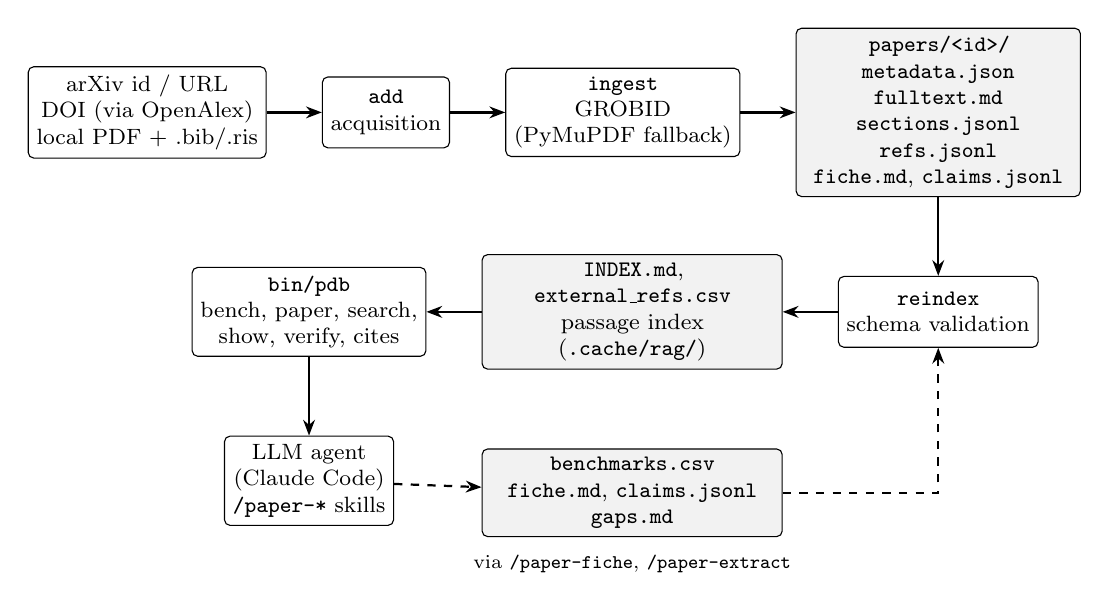
\begin{tikzpicture}[
  node distance=5mm and 7mm,
  box/.style={draw, rounded corners=2pt, align=center, font=\footnotesize,
              minimum height=9mm, inner sep=3pt, fill=white},
  store/.style={box, fill=gray!10},
  arr/.style={-{Stealth[length=2mm]}, thick}]
  \node[box] (src) {arXiv id / URL\\DOI (via OpenAlex)\\local PDF + .bib/.ris};
  \node[box, right=of src] (add) {\cmd{add}\\acquisition};
  \node[box, right=of add] (ingest) {\cmd{ingest}\\GROBID\\(PyMuPDF fallback)};
  \node[store, right=of ingest, text width=34mm] (papers)
    {\cmd{papers/<id>/}\\\cmd{metadata.json}\\\cmd{fulltext.md}\\\cmd{sections.jsonl}
     \\\cmd{refs.jsonl}\\\cmd{fiche.md}, \cmd{claims.jsonl}};
  \node[box, below=10mm of papers] (reindex) {\cmd{reindex}\\schema validation};
  \node[store, left=of reindex, text width=36mm] (derived)
    {\cmd{INDEX.md}, \cmd{external\_refs.csv}\\passage index\\(\cmd{.cache/rag/})};
  \node[box, left=of derived] (pdb) {\cmd{bin/pdb}\\bench, paper, search,\\show, verify, cites};
  \node[box, below=10mm of pdb] (agent) {LLM agent\\(Claude Code)\\\cmd{/paper-*} skills};
  \node[store, below=10mm of derived, text width=36mm] (bench)
    {\cmd{benchmarks.csv}\\\cmd{fiche.md}, \cmd{claims.jsonl}\\\cmd{gaps.md}};
  \draw[arr] (src) -- (add);
  \draw[arr] (add) -- (ingest);
  \draw[arr] (ingest) -- (papers);
  \draw[arr] (papers) -- (reindex);
  \draw[arr] (reindex) -- (derived);
  \draw[arr] (derived) -- (pdb);
  \draw[arr] (pdb) -- (agent);
  \draw[arr, dashed] (agent) -- (bench);
  \node[below=1mm of bench, font=\scriptsize] {via \cmd{/paper-fiche}, \cmd{/paper-extract}};
  \draw[arr, dashed] (bench.east) -| (reindex.south);
\end{tikzpicture}
\caption{Data flow. Solid arrows are automatic; dashed arrows go through the agent, which
writes reading notes, atomic evidence and benchmark rows from the extracted text.}
\label{fig:pipeline}
\end{figure}

\subsection{Acquisition and ingestion}

\cmd{bin/add.py} fetches an arXiv paper (metadata through the \gl{API}{API}, then the \gl{PDF}{PDF}), resolves a
\gl{DOI}{DOI} to its arXiv version through OpenAlex \citep{priem2022openalex}, or copies a local PDF.
Paywalled papers are dropped in by hand: the tool bypasses no access control.

\cmd{bin/ingest.py} sends each PDF to \gl{GROBID}{GROBID} \citep{grobid}, which returns a \gl{TEI}{TEI} structure
(header, sections, figures, bibliography). Without GROBID, a PyMuPDF fallback splits the text
heuristically on numbered headings and records this in the metadata. The pipeline then
applies, in order:
\begin{itemize}
  \item \emph{metadata merging} by order of trust: publisher citation export, then arXiv,
    then GROBID. An unknown field stays \cmd{null};
  \item \emph{cleaning}: repeated headers and footers, page numbers, bibliography moved out
    of the body into \cmd{refs.jsonl};
  \item \emph{repair of lost ligatures} («~classi cation~» for «~classification~»): a word
    is rejoined only if the result is known to the corpus or to a built-in list and the
    fragment is not;
  \item \emph{tables}: a table for which GROBID kept only the caption goes through two
    successive fallbacks. PyMuPDF first looks for it on its page (ruled tables). Docling
    \citep{auer2024docling} comes next, on request (\cmd{ingest --reparse --tables
    docling}), with optional optical character recognition (\gl{OCR}{OCR}) for tables published as
    images. A reconstructed body is labelled ``reconstructed by PyMuPDF / Docling: to be
    checked'', and a table left empty is reported by \cmd{pdb status}. Each table keeps its
    page, its frame on the page (\cmd{bbox}) and the extractor that produced it
    (\cmd{table\_source}). Seven quality signals, computed at read time, flag suspect tables:
    empty cells, a varying number of cells from one row to another, no header, doubtful OCR
    characters, glued numbers, lost columns, and a caption matched by rank rather than by
    number (\cmd{pdb status --tables});
  \item \emph{misclassified paragraphs}: a paragraph that GROBID took for a figure is
    returned to the body when it looks like prose.
\end{itemize}
Ingestion is idempotent, and a re-extraction (\cmd{--force}, or \cmd{--reparse} from the
stored TEI) never overwrites a \gl{fiche}{reading note} already written nor a classification corrected
by hand.

\subsection{Data model}
\label{sec:data}

Each paper becomes a folder \cmd{papers/<paper\_id>/}. The identifier is stable and readable
(\cmd{arxiv-<id>-<slug>} or \cmd{<year>-<author>-<slug>}). The extracted text exists in two
forms: \cmd{fulltext.md}, human-readable, and \cmd{sections.jsonl}, one line per section with
its type (abstract, section, figure, table) and its page. The latter is the raw material of
the \gl{passage}{passage} index.

The file \cmd{benchmarks.csv} has one row per reported configuration: a paper that presents
three variants yields three rows. Besides the measurement columns (model, platform,
quantisation, \gl{FPS}{FPS}, \gl{GOPS}{GOPS}, latency, power, \gl{LUT}{LUT}, \gl{DSP}{DSP}, \gl{BRAM}{BRAM}, dataset, \gl{toolflow}{toolflow}), three columns
are used to judge each value:
\begin{itemize}
  \item \cmd{source\_section}: section, table or figure of origin;
  \item \cmd{confidence}: \cmd{high} (read from a table), \cmd{medium} (read from the text)
    or \cmd{low} (inferred, to be rechecked);
  \item \cmd{power\_scope}: \gl{scope}{scope} of the reported power (\cmd{chip}, \cmd{board},
    \cmd{board-dynamic}, \cmd{estimated}, \cmd{unspecified}). Two powers with different
    scopes cannot be compared: a board can draw several watts at idle, which a ``board''
    measurement includes and a ``chip'' measurement excludes.
\end{itemize}
These twenty columns do not say everything about the conditions of a measurement. Seven
\emph{optional} columns, added on request (\cmd{pdb bench --add-columns}), complete them: the
passage that contains the value (\cmd{chunk\_id}), the exact definition of the metric, the
evaluated split, the input resolution, the batch size, the measurement protocol and the value
as written when it was converted. When absent, an optional column is \nr{}: an existing base
stays valid without migration, and no current row fills them yet. \cmd{pdb bench --check}
verifies that every number of a row that cites a passage does appear in that passage, and
\cmd{pdb bench --comparable} groups the rows by task, dataset, split and metric (or power
scope) before any comparison between papers. It flags the conditions that vary within a
group, those that are missing, and the impossible comparisons. On the fpga base, the 56
detection rows on COCO, from 7 papers, form 9 groups, none of which gathers two papers: none
of these values is directly comparable to another.

Reading notes (\cmd{fiche.md}) follow a fixed template (problem, method, results,
limitations, relevance) with a mandatory ``reading status'' section that separates what was
read from what was inferred. They are written by the \gl{agent}{agent} (\cmd{/paper-fiche} command) and
reviewed by the user.

A note summarises; its numbers carry their source, but its qualitative statements (method,
limitation, hypothesis) do not. The \cmd{claims.jsonl} file of a paper holds its
\gl{claim}{atomic evidence}: one statement per line, with its type (result, method, limitation,
hypothesis, context), its voice (the authors, or a deduction by the reader), the source
passage, the exact excerpt that carries it, and optionally its conditions and the benchmark
row that transcribes it. The \cmd{/paper-extract} skill writes them. At every reindex, each
excerpt is checked by \cmd{verify} against its passage: an absent excerpt or one with wrong
numbers is an error, and the reindex fails. A number of the statement that is absent from the
source section is flagged. First trial, on the FINN paper: 32 items, 32 verified excerpts, a
single note, a legitimate one (value taken from a neighbouring passage); an error introduced
on purpose (altered number, wrong passage) is rejected. The other papers have not been
processed yet, and retrieval does not read this evidence yet.

\subsection{Several bases}
\label{sec:bases}

The same code serves several knowledge bases, one per topic. The repository holds three
(table~\ref{tab:bases}): the \emph{fpga} base of the use case, which serves as the reference
and now covers a thesis on safe and certifiable embedded \gl{AI}{AI} on FPGA; a \emph{drone} base
(embedded vision on drones: detection, accelerators, co-design of computing, energy and
flight), created later on a neighbouring topic; and a \emph{stage} base, on embedded continual
learning on microcontrollers (\gl{MCU}{MCU}) for predictive maintenance, built from the bibliography
of an internship. The latter is the furthest from the original domain: its founding papers
(Mahalanobis, 1936, scanned and run through \gl{OCR}{OCR}) have no hardware measurement, and its
benchmarks concern bearing and turbine datasets rather than accelerators. The repository root
holds only the code. Each base is a \cmd{bases/<name>/} folder with its own papers,
\cmd{benchmarks.csv}, gap map, \gl{passage}{passage} index and caches; the commands, the Python
environment and the \gl{agent}{agent}'s skills are links to the code.

\begin{table}[ht]
\centering
\caption{The three bases on 03/10/2026 (output of \cmd{pdb base list} and \cmd{pdb status}).}
\label{tab:bases}
\small
\begin{tabular}{@{}lrrrr@{}}
\toprule
Base & Papers & Notes done & Benchmark rows & Indexed passages \\
\midrule
fpga (reference) & 101 & 101 & 299 & 8\,601 \\
drone & 87 & 86 & 352 & 5\,361 \\
stage & 56 & 56 & 100 & 3\,640 \\
\bottomrule
\end{tabular}
\end{table}

What depends on the domain fits in two files per base. \cmd{base.json} declares the watch
axes and regular-expression rules that put a paper in an axis, give it tags and decide
whether it is on topic (the last test is used by discovery). \cmd{profile.md} describes the
topic and scope (included, excluded) in prose; the \cmd{/base-profile} skill proposes
refinements drawn from the reading notes, and writes nothing without approval. Each base also
has its own \cmd{CLAUDE.md}, which carries the domain's working rules: for the drone base,
stating the power range of a result, or telling ground-to-air from air-to-air detection
apart. The columns of \cmd{benchmarks.csv} remain common to all bases; the optional columns
(section~\ref{sec:data}) are added base by base. The figures of \cmd{pdb plot} adapt as well:
a \cmd{plot} block in \cmd{base.json} declares the tasks and platform families to
distinguish and the figures to omit. The stage base, with no hardware measurements and no
question sets, has 8 figures, versus 16 for fpga. \cmd{pdb plot --check} proposes this block
from the content of the base, and \cmd{reindex} regenerates the figures that have become
stale.

The active base follows from the context: the \cmd{\$PDB\_ROOT} variable (set by
\cmd{pdb --base <name>}), otherwise \cmd{\$PDB\_BASE}, otherwise the first folder containing
\cmd{base.json} walking up from the current directory, otherwise the default base of a local
registry (\cmd{\textasciitilde/.config/pdb/bases.json}), otherwise the reference base. Two
agent sessions opened in two bases therefore each work on their own.

Bases stay separate, but a paper can move from one to another. \cmd{pdb base scan} searches
the other bases for papers useful to the current one: those it already cites without having
them, those that match its rules, and references cited on both sides. \cmd{pdb base import}
copies a paper without re-extracting it and sends its reading note back for review, since
its relevance depends on the topic of the receiving base.

\subsection{Modules}

\begin{table}[ht]
\centering
\caption{Main modules of \cmd{lib/}. Everything is written in Python; only dense retrieval,
the GPU engine, the figures and the visualisation have optional dependencies.}
\label{tab:modules}
\small
\begin{tabularx}{\linewidth}{@{}lL@{}}
\toprule
Module & Role \\
\midrule
\cmd{tei.py}, \cmd{doc.py}, \cmd{pdftext.py} & reading GROBID output, common representation, PyMuPDF fallback \\
\cmd{ligatures.py}, \cmd{tables.py}, \cmd{docling\_tables.py} & ligature repair, table reconstruction (PyMuPDF, then Docling), quality signals \\
\cmd{citation.py}, \cmd{openalex.py} & \cmd{.bib}/\cmd{.ris} exports, OpenAlex client with cache \\
\cmd{schema.py} & data-model validators, the only place where it is coded \\
\cmd{refs.py} & reference matching (arXiv, DOI, normalised title), internal citations \\
\cmd{query.py} & structured queries without LLM (\cmd{bench}, \cmd{paper}, \cmd{cites}), \cmd{--check}, comparable groups \\
\cmd{rag.py} & passages (tables split by rows), BM25, dense index, fusion, reranking, quotation checking; optional Qwen engine \\
\cmd{claims.py} & checking of atomic evidence (\cmd{claims.jsonl}) against its passage \\
\cmd{rag\_qwen.py}, \cmd{rag\_models.py} & GPU engine: pinned Qwen3 models (shared with \cmd{pdb search}), FTS5 evidence index of \cmd{pdb rag} \\
\cmd{rag\_external.py} & staged open-access acquisition (OpenAlex, arXiv), import after approval \\
\cmd{evaluation.py} & evaluation bench (\cmd{pdb eval}): extraction, retrieval, \cmd{verify}, timings, final answers \\
\cmd{agentlog.py}, \cmd{agentcost.py} & subagent log, cost calibrated on Claude Code, savings from delegation \\
\cmd{status.py} & state of the base and next actions \\
\cmd{base.py}, \cmd{registry.py} & active base, reading \cmd{base.json}, classification by its rules; registry of bases \\
\cmd{bases.py}, \cmd{xbase.py}, \cmd{vizbases.py} & creating and checking bases, scan and import across bases, Bases tab of the visualisation \\
\cmd{plotdata.py}, \cmd{plotfig.py}, \cmd{plotrun.py} & static figures (\cmd{pdb plot}): benchmarks, evaluation, corpus; regeneration of stale figures \\
\cmd{graph.py}, \cmd{lineage.py}, \cmd{vizfig.py}, \cmd{embed.py} & 3D visualisation and citation lineage (secondary tool) \\
\bottomrule
\end{tabularx}
\end{table}

All commands go through a single entry point, \cmd{bin/pdb}. Their output follows the same
conventions: \gl{CSV}{TSV} by default, a header line without banner, notes prefixed by \cmd{\#}, short
paper identifiers (\cmd{1612.07119}, \cmd{2022-feng}) with their legend at the bottom, and an
exit code that distinguishes ``results'', ``no result'' and ``argument error''.

\section{The retrieval layer (RAG)}
\label{sec:rag}

\subsection{A RAG without generation}

In a \emph{Retrieval-Augmented Generation} system \citep{lewis2020rag}, the \gl{LLM}{LLM} receives,
together with the question, the \gl{passage}{passages} of a corpus that answer it, and writes from them.
PaperDatabase separates the two halves. The \cmd{bin/pdb} commands do the retrieval,
deterministically and without calling an LLM. The \gl{agent}{agent} calls them, reads their output and
writes only when a synthesis is needed. This choice adds neither an \gl{API}{API} key nor a cost: the
generation is done by the agent already in use.

Three goals guide the design, in order of priority: \emph{verifiability} (every returned
item carries a replayable source), \emph{token economy} (answering without reading full
texts), and \emph{access by meaning} (finding ``continual learning'' when searching for
``incremental learning'', which \cmd{grep} cannot do).

\begin{table}[ht]
\centering
\caption{Three query levels, from cheapest to most expensive. One moves up a level only if
the previous one is not enough. Costs measured on the current corpus.}
\label{tab:niveaux}
\small
\begin{tabularx}{\linewidth}{@{}lllL@{}}
\toprule
Level & Source & LLM & Typical cost \\
\midrule
N0 -- structured query & \cmd{benchmarks.csv}, metadata & no & 100--500 tokens \\
N1 -- passage retrieval & passage index & no & 400--800 tokens, +300 per opened passage \\
N2 -- synthesis & N0 and N1 outputs only & yes & that of the writing \\
\bottomrule
\end{tabularx}
\end{table}

An N0 or N1 output is often already an answer: a filtered table or three sourced passages
are enough for a factual question, and the agent can pass them on without rephrasing. Level
N2 adds no information: it links what N0 and N1 returned, and labels its inferences as such.

\subsection{Passage chunking}

The starting unit is an entry of \cmd{sections.jsonl}, which already follows paragraphs. An
entry longer than 250 words is split into 200-word windows with a 40-word overlap, because
\gl{embedding}{embedding} models truncate beyond 256 to 512 tokens. Each passage gets a replayable
identifier, \cmd{<section>.<k>} (for example \cmd{1612.07119\#019.3}), and keeps its paper,
section, page and the \gl{SHA}{SHA-1} hash of its text. The indexed text is prefixed with the section
title, which adds context without changing the returned text. A table longer than 250 words
is split differently: by whole rows, each window repeating the abridged caption and the header
row, so that a value is never separated from its unit or its column. Across the three bases,
181 tables are concerned; they yield 610 windows (median 186 words) with no loss of words.
The fpga base now has 8\,601 passages.

\subsection{Two indexes and a fusion}

\paragraph{Lexical index.} A hand-written \gl{BM25}{BM25} \citep{robertson2009bm25} ($k_1 = 1.5$,
$b = 0.75$, lower-case alphanumeric tokens) finds exact terms: board names (\cmd{ZCU104}),
model names (\cmd{YOLOv5n}), acronyms and numbers.

\paragraph{Dense index.} The \cmd{BAAI/bge-small-en-v1.5} model \citep{xiao2024cpack}
(384 dimensions), loaded with sentence-transformers \citep{reimers2019sbert}, encodes each
passage into a normalised vector. It finds paraphrases and, to some extent, queries in
another language. The query gets the instruction prefix recommended for the model; passages
do not.

\paragraph{Fusion.} Both rankings are merged by Reciprocal Rank Fusion
\citep{cormack2009rrf}:
\begin{equation}
  \operatorname{score}(d) = \sum_{i \in \{\text{BM25},\,\text{dense}\}}
    \frac{1}{60 + \operatorname{rank}_i(d)} .
\end{equation}
This method does not depend on score scales, needs no tuning and stays deterministic. Ties
are broken by the smallest identifier: the same query on the same index always gives the
same ranking.

\paragraph{Absolute relevance.} The \gl{RRF}{RRF} score is a rank, not a relevance measure:
\cmd{search} always returns $k$ passages, even when the base does not cover the topic. The
output shows the cosine between the query and each passage. A first version warned
(\cmd{\# pertinence faible}, ``low relevance'') when the best cosine fell below a threshold
calibrated by hand on a few queries. The evaluation bench showed that this warning never
fired, and that no threshold, neither on the cosine nor on a \gl{crossenc}{cross-encoder} score, separated
out-of-corpus questions from the others (section~\ref{sec:horscorpus}). It was therefore
removed, because it gave false reassurance: the agent judges, from the snippets, whether the
base answers, and says so otherwise instead of filling the gap.

\paragraph{Reranking (option).} \cmd{--rerank} reorders the top 30 results with the
\cmd{ms-marco-MiniLM-L-6-v2} cross-encoder, a MiniLM \citep{wang2020minilm} trained on
\gl{MSMARCO}{MS MARCO} \citep{nguyen2016msmarco} following \citet{nogueira2019rerank}. It costs about 1.4\,s
per warm search. It is not enabled by default, for the reasons given in
section~\ref{sec:eval}.

\paragraph{Storage.} Vectors are stored in \cmd{.cache/rag/<model>.npz}, keyed by
\cmd{chunk\_id:sha1}. Updates are incremental: only new or modified passages are encoded
(about 8~min for a full build of the 8\,601 passages of the fpga base on \gl{CPU}{CPU}, i.e.\ 18
passages per second; 0.2\,s with no change). Passages and BM25 are recomputed by each command
in under a second. Without sentence-transformers, or if the index is stale, \cmd{search} falls
back to lexical only and says so. At this scale, an exhaustive numpy search takes a few
milliseconds: a dedicated vector database would bring nothing before roughly $10^5$ passages
(estimate, not measured).

\subsection{Commands}

\cmd{pdb bench} filters \cmd{benchmarks.csv} (substrings, numerical bounds, non-empty columns,
sorting, aggregation with \cmd{--count}). The source columns (\cmd{source\_section},
\cmd{confidence}, \cmd{power\_scope}) are always shown, even when not requested, and a
low-confidence row is prefixed with \cmd{!}.

\begin{lstlisting}
$ bin/pdb bench --platform kv260 --cols model,quantization,fps,power_w
paper       model                  quantization  fps  power_w  power_scope  source_section  confidence
2507.18174  YOLOv5 (variante n/r)  INT8          9    3.5      unspecified  Table I         high
# ids: 2507.18174=arxiv-2507.18174-real-time-object-detection-classification
\end{lstlisting}

\cmd{pdb search} returns one line per passage: identifier, section, page, cosine and a
snippet of about 160 characters centred on the rarest query term (rare terms in guillemets).
Real output, shortened snippets:

\begin{lstlisting}
$ bin/pdb search "power measured at the wall versus the FPGA rails" -k 3
chunk               section                       page  cos   snippet
1612.07119#022.0    5. EVALUATION / 5.2.2. …      8     0.78  …both the «wall» «power» and «FPGA» «power» readings…
2025-hozhabr#051.1  V. RESULTS ANALYSIS … / B. …  31    0.77  …computational «power», or throughput, «measured» in…
1612.07119#019.3    5. EVALUATION / 5.1. …        7     0.73  …PMBus interface to monitor the «FPGA» «power» supply «rails»…
\end{lstlisting}

\cmd{pdb show} prints the exact text of a passage with its header (section, page, start of
the SHA-1) and, on request, its neighbours. \cmd{pdb verify} checks that a quotation appears
in the cited passage. Both texts are normalised (ligatures, case, hyphenation, everything
that is neither letter nor digit), then compared by exact search or, failing that, by the
best \cmd{difflib} window. The verdict is one of five (the tool's labels are in French):
\begin{itemize}
  \item \cmd{OK}: the quotation appears as is, after normalisation;
  \item \cmd{APPROX}: similarity of at least 0.85 (close paraphrase);
  \item \cmd{NOMBRES} (``numbers''): similarity of at least 0.85, but the numbers of the
    quotation are not those of the passage;
  \item \cmd{ABSENT}: similarity below 0.85;
  \item \cmd{MODIFIÉ} (``modified''): the passage has changed since its SHA-1 was recorded.
\end{itemize}
Only \cmd{OK} and \cmd{APPROX} give a zero exit code. The \cmd{NOMBRES} status comes from the
evaluation bench. In a long sentence, a changed number keeps the similarity above the
threshold, and the first version thus accepted every quotation with an altered number
(section~\ref{sec:evalverify}). The added check requires the numbers of the quotation to
form a contiguous run of the passage's numbers. Each must appear with its neighbouring
words: ``Section 3 reviews'' is rejected even if the passage contains a 3 elsewhere. Since
normalisation removes punctuation, this check is also what tells ``94.9\,\%'' from
``949\,\%''.

A quotation absent from the cited passage but present elsewhere in the same paper is
reported with the identifier where it was found, and the command exits with an error: the
source was wrong.

\begin{lstlisting}
$ bin/pdb verify 1612.07119#019.3 "P-wall using a wall-power meter for the whole board power consumption"
APPROX  0.95  1612.07119#019.3
\end{lstlisting}

Finally, \cmd{pdb paper} gives the identity of a paper (authors, venue, \gl{preprint}{preprint} or not,
note status), and \cmd{pdb cites} / \cmd{cited-by} walk the citation graph internal to the
corpus, rebuilt by matching references on arXiv identifier, \gl{DOI}{DOI} or normalised title.

\subsection{Answer protocol: the \cmd{/paper-ask} skill}
\label{sec:paperask}

The \cmd{/paper-ask} \gl{skill}{skill} gives the agent a fixed procedure and only allows it to use the
\cmd{bin/pdb} commands and file reading:
\begin{enumerate}
  \item before any search, state 2 to 5 \gl{exigence}{requirements}, what a complete answer must
    establish (a value, a platform, a condition, a comparison), without going further than
    the question asks;
  \item numerical question: \cmd{pdb bench} first (N0), and \cmd{bench --comparable} before
    comparing two papers;
  \item otherwise, or in addition: \cmd{pdb search --rerank} with one or two English
    phrasings; if no snippet answers, say that the base probably does not cover the topic
    instead of filling the gap;
  \item \cmd{pdb show} on 2 or 3 passages at most, never on the full text;
  \item answer with \cmd{[chunk\_id]} citations, and \cmd{pdb verify} on every verbatim
    quotation: an \cmd{ABSENT} quotation is removed, a \cmd{NOMBRES} quotation is corrected
    from the exact text or removed, a wrong identifier is corrected, and an \cmd{APPROX}
    quotation is kept only if presented as a paraphrase;
  \item mark each requirement \cmd{couvert} (``covered'', verified passage), \cmd{partiel}
    (``partial'', neighbouring passage: other platform, other batch, other power scope) or
    \cmd{absent}, and derive the \gl{verdict}{verdict} from them: \cmd{suffisant} (``sufficient'') if all are covered,
    \cmd{absent} if none is, \cmd{partiel} otherwise;
  \item imposed structure: the verdict and the requirements first, then \textbf{Read}
    (sourced), \textbf{Inferred}, \textbf{Not found in the base}, flagging low-confidence
    values, preprints and heterogeneous \gl{scope}{power scopes}.
\end{enumerate}
The verdict moves the question ``does the base cover this topic?'' away from a retrieval
score, which does not settle it (section~\ref{sec:horscorpus}), toward the content of the
passages read. An \cmd{absent} verdict concerns the base, not the literature: the answer says
so and suggests \cmd{/paper-discover}. A \cmd{--record} mode writes the answer as \gl{JSON}{JSON}, in
the form of cited statements, for the evaluation of answers (section~\ref{sec:answers}).

\subsection{An optional GPU engine and open-access acquisition}
\label{sec:qwen}

\paragraph{Engine.} A second retrieval chain was developed in parallel, for a machine with a
\gl{GPU}{GPU} (measurements made on a 32~GB RTX 5090): \cmd{Qwen3-Embedding-4B} for the dense index
and \cmd{Qwen3-Reranker-4B} for \gl{reranking}{reranking}, in \gl{BF16}{BF16} with pinned model revisions. It is now an
\emph{optional engine of \cmd{pdb search}}: it encodes exactly the same passages, with the same
identifiers, so that \cmd{show}, \cmd{verify}, \cmd{/paper-ask} and the evaluation of answers
do not change. The \gl{CPU}{CPU} engine remains the default. \cmd{pdb gpu on} enables the GPU engine
for the machine (a setting outside the bases), downloads the models and reindexes; \cmd{--gpu}
or \cmd{--cpu} forces one for a single search. Without CUDA, without the required libraries
or without Qwen vectors for the base, \cmd{search} stays on the CPU and says so: a question
never fails for lack of a GPU. \cmd{pdb eval --rag --gpu} writes a report with the same keys
as the CPU engine, which makes it possible to compare the two engines with \cmd{--compare}.

The \cmd{bin/pdb rag} command keeps what remains specific to the original chain: an SQLite
index (\gl{FTS5}{FTS5} and Qwen vectors) of \emph{typed} evidence, which holds, next to the abstracts,
sections, tables and figures of the original text, the finished \gl{fiche}{reading notes} and the rows of
\cmd{benchmarks.csv}, each labelled as transcription or note. A note or a
\gl{benchmark}{benchmark row} is for navigation, and the agent must go back to the original passage
(\cmd{rag evidence ID --parent}) before quoting. \cmd{rag benchmarks} filters numbers with no
cap on results; \cmd{rag check-answer} checks, for an answer recorded in
\gl{JSON}{JSON}, that each quoted excerpt appears in the cited evidence, without yet checking
numbers as \cmd{verify} does. The \cmd{/paper-research} skill frames this route.

\paragraph{Acquisition.} When the corpus is not enough, \cmd{rag acquire} looks for
open-access full texts (OpenAlex, arXiv), downloads them into a private staging directory,
extracts them and deduplicates them by DOI, arXiv identifier and document hash. Nothing
enters the base at this stage: the agent presents each retained paper (title, year,
excerpt) and calls \cmd{rag approve} only for those the user accepts. An imported paper gets
a \cmd{todo} note and never overwrites a paper already present. A budget bounds each session:
8 searches, 8 \gl{PDF}{PDFs}, 50~MB per PDF, 200~MB and 15 minutes in total. An unavailable PDF is
treated as a limitation of the search, not as evidence of absence.

\paragraph{Measurement.} The two engines were compared on the question sets of
section~\ref{sec:eval}, with the same expectations and the same metrics
(table~\ref{tab:qwen}). This comparison dates from 26/09/2026, on the 28-paper corpus, with
the original \cmd{pdb rag} chain: it was redone neither on the current corpus nor with the
engine built into \cmd{pdb search}, as the machine used for the later measurements has no GPU.

\begin{table}[ht]
\centering
\caption{CPU engine (bge-small) versus GPU engine (Qwen3), same question sets, 28-paper
corpus. Bold: best value per set.}
\label{tab:qwen}
\small
\begin{tabular}{@{}llccccc@{}}
\toprule
Set & Engine & recall@5 & recall@10 & MRR & nDCG@10 & s / question \\
\midrule
dev (20)     & bge-small hybrid + reranking & \textbf{1.00} & \textbf{1.00} & \textbf{0.85} & \textbf{0.46} & $\sim$1.4 \\
             & Qwen hybrid                  & 0.90 & 0.90 & 0.78 & 0.37 & 0.7 \\
             & Qwen hybrid + reranking      & 0.80 & 0.80 & 0.76 & 0.35 & 3.7 \\
\midrule
holdout (25) & bge-small hybrid + reranking & 0.80 & 0.80 & \textbf{0.78} & \textbf{0.41} & $\sim$1.4 \\
             & Qwen hybrid + reranking      & \textbf{0.88} & \textbf{0.92} & 0.75 & 0.35 & 3.3 \\
\midrule
FR (8)       & bge-small dense (best mode)  & 0.62 & 0.75 & 0.46 & 0.19 & 0.1 \\
             & Qwen dense                   & \textbf{1.00} & \textbf{1.00} & 0.63 & 0.22 & 0.7 \\
             & Qwen hybrid + reranking      & \textbf{1.00} & \textbf{1.00} & \textbf{0.88} & \textbf{0.31} & 3.8 \\
\bottomrule
\end{tabular}
\end{table}

The only clear gap is French: Qwen retrieves all 8 questions without rephrasing them in
English. On the held-out set, it gains 2 questions out of 25 at \gl{recall}{recall@5}, with a comparable
\gl{MRR}{MRR}. On the dev set, it does worse, which is partly expected since this set was used to tune
the first engine. Its lexical channel (FTS5) is weaker than the first engine's BM25 (dev
0.80 versus 0.95; French 0.00). The Qwen reranker is also the best out-of-corpus signal
measured (section~\ref{sec:horscorpus}). It comes at a cost: a GPU (each model takes about
8~GB), and models reloaded for each query, i.e.\ 3 to 4\,s per question with reranking. The
CPU engine therefore remains the default; the GPU engine is an aid for French questions and
vocabulary mismatch.

\section{What the software brings}
\label{sec:apports}

\paragraph{Token savings.} Table~\ref{tab:tokens} compares, for four common tasks, reading
the files directly and going through the commands. Orders of magnitude are measured on the
current corpus (file size divided by four).

\begin{table}[ht]
\centering
\caption{Token cost of common tasks (orders of magnitude).}
\label{tab:tokens}
\small
\begin{tabularx}{\linewidth}{@{}lLl@{}}
\toprule
Task & Without the retrieval layer & With \\
\midrule
A number on a platform & read the whole \cmd{benchmarks.csv}: $\sim$27\,000 & filtered \cmd{bench}: 100--400 \\
Find where a topic is discussed & \cmd{grep} over sections, which misses synonyms & \cmd{search -k 8}: $\sim$600 \\
Read the evidence for a claim & open \cmd{fulltext.md}: $\sim$12\,000 (median) & \cmd{show} on 1 to 3 passages: 300--900 \\
Check a quotation & reread the passage & \cmd{verify}: $\sim$20 \\
\bottomrule
\end{tabularx}
\end{table}

\paragraph{Verifiability.} Every returned item can be replayed: a \gl{passage}{passage} by its identifier
(\cmd{show}) and its page in the \gl{PDF}{PDF}, a quotation by \cmd{verify}, a number by its
\cmd{bench} row and source section, a ranking by the determinism of the fusion. An empty
result is presented as a statement about the base, not about the literature. Paraphrases,
cross-paper connections and inferences cannot be checked automatically: the \gl{agent}{agent} must label
them as inferred.

\paragraph{Beyond retrieval.} The same base serves other PhD-preparation tasks:
\begin{itemize}
  \item extracted references feed \cmd{external\_refs.csv}, which ranks works missing from
    the base by the number of corpus papers that cite them: these are the next readings;
  \item \cmd{pdb discover} (\cmd{/paper-discover}) queries OpenAlex (incoming citations,
    search by axis or by \gl{gap}{gap}) and proposes candidates, added only with the user's approval;
  \item \cmd{/paper-gaps} keeps a map of uncovered areas (\cmd{gaps.md}), each entry
    supported by paper identifiers;
  \item state-of-the-art reviews in \LaTeX{} were written by the agent from the notes of the
    fpga and drone bases (sections by axis, glossaries, links to the papers), then proofread;
    every statement in them points to a paper of the base;
  \item a local visualisation app (3D corpus graph, citation timeline) gives the user an
    overview; the agent does not use it;
  \item \cmd{pdb plot} produces static figures (PNG, PDF or SVG) from
    \cmd{benchmarks.csv}, the latest \cmd{pdb eval} report and the corpus metadata:
    throughput versus power, \gl{GOPS}{GOPS}/W by precision, \gl{FPGA}{FPGA} resources, accuracy versus
    throughput, retrieval quality, years, axes, citations, gaps. Each figure states its
    source and sample size in a footer (for example 82 rows out of 299, \nr{} values being
    excluded), and \cmd{figures/manifest.json} lists them. Figure~\ref{fig:fpspower} is an
    example; heterogeneous \gl{scope}{power scopes} are distinguished there rather than mixed.
\end{itemize}

\begin{figure}[ht]
\centering
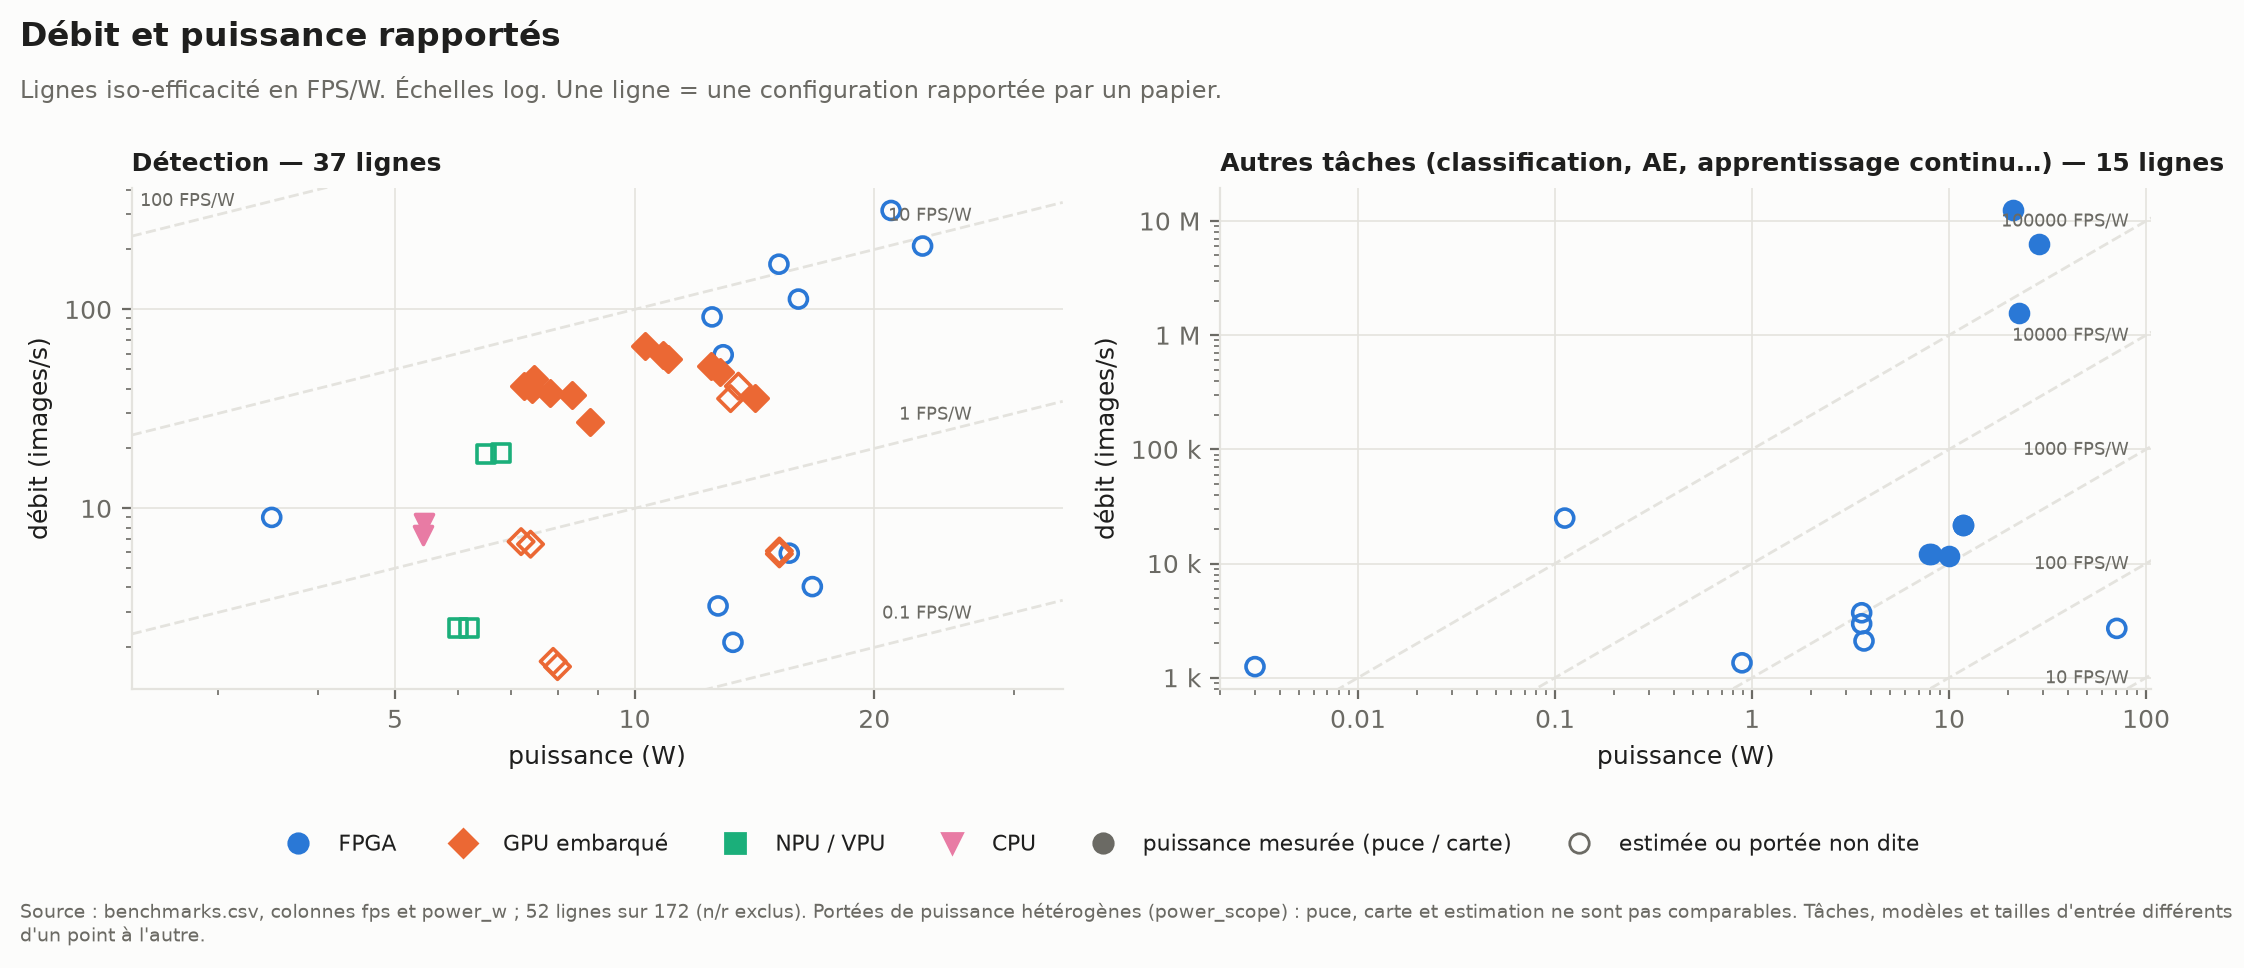
\includegraphics[width=\linewidth]{bench_fps_power.png}
\caption{Output of \cmd{pdb plot bench} on the fpga base: reported throughput and power, one
configuration per point (82 rows of \cmd{benchmarks.csv} out of 299), detection on the left,
other tasks on the right. Filled markers: measured power; hollow: estimated or unspecified
scope. Points cannot be compared with one another without reading the scope of the
measurement (section~\ref{sec:data}, \cmd{bench --comparable}).}
\label{fig:fpspower}
\end{figure}

\paragraph{Delegating to subagents.}
\label{sec:delegation}
The main agent can hand a task to a \gl{sousagent}{subagent} that starts without its context: one
note per agent, one paper to extract, a DOI lookup. The repository rules set the model by
task: the lightest for mechanical work (adding, reindexing, checking metadata), an
intermediate one for reading and extraction, the most capable for synthesis and judgement. Two
agents never write the same file, and \cmd{benchmarks.csv}, \cmd{INDEX.md} and the reindex
stay with the main agent, which verifies what is reported to it. To know whether this pays,
a Claude Code \cmd{SubagentStop} \gl{hook}{hook} logs every subagent (tokens, cost, duration, tools) in
\cmd{.cache/agents.jsonl}, and \cmd{pdb agents --report} summarises it. The cost derived from
the transcripts underestimated output tokens; it is calibrated on the cost that Claude Code
counts for the session. Over 72 logged subagents (126~M tokens, \$81), delegation would have
saved about 59~\% of the cost of the same work done directly. This figure is an
\emph{estimate}: the same turns at the main agent's rate, plus rereading the work at each
following turn.

To calibrate it, the same task (three reading notes on YOLO detectors of the drone base) was
done twice in fresh sessions, directly and then delegated to three subagents in parallel
(table~\ref{tab:delegation}). The model predicts \$2.21 for the direct session, which cost
\$2.30 (a 4~\% gap). Delegation cost 41~\% less and took 59~\% less time. The trial is single,
and the two sessions did not produce the same work: directly, the notes are longer and include
9 more benchmark rows. Part of the gap therefore comes from the work, not only from the rate,
and quality was not scored. The experiment also revealed a defect of the log: the hook ran
before the last turn of the subagent was written, which was missing from the count; it now
rereads the transcript until it is complete.

\begin{table}[ht]
\centering
\caption{Paired experiment: three reading notes, direct and delegated (03/10/2026, a single
trial).}
\label{tab:delegation}
\small
\begin{tabular}{@{}lrr@{}}
\toprule
 & Direct & Delegated \\
\midrule
Cost counted by Claude Code & \$2.30 & \$1.35 (0.46 + 0.89 for the subagents) \\
Duration & 324\,s & 133\,s \\
Main agent turns & 29 & 6 (+ 24 for the 3 subagents) \\
Main context at end of session & 139k tokens & 54k tokens \\
\cmd{benchmarks.csv} rows / size of the notes & 24 / 23.5k chars & 15 / 17.8k chars \\
\bottomrule
\end{tabular}
\end{table}

\paragraph{State of the corpus.} As of 3 October 2026, the fpga base has 101 papers, all with a
finished \gl{fiche}{reading note}, 299 \gl{benchmark}{benchmark rows}, 8\,601 indexed passages and 37 recorded gaps, 29
of them supported by corpus papers (output of \cmd{pdb status}). The corpus has more than
doubled since the previous version of this text (45 papers, 3\,479 passages), largely with
papers on the safety and certification of embedded AI; the notes and benchmark rows of the
new papers were written by subagents, then verified by the main agent.

\section{Tests and evaluation}
\label{sec:tests}

\subsection{Unit tests}

The suite (\cmd{bin/pdb test}) has 286 tests in 26 files. It runs in under 30 seconds,
without \gl{GROBID}{GROBID} and without \gl{embedding}{embedding} models, thanks to deterministic stand-ins
(table~\ref{tab:tests}):
\begin{itemize}
  \item a real GROBID (0.8.1) \gl{TEI}{TEI} output, kept as a fixture, for parsing;
  \item a fake encoder and \gl{crossenc}{cross-encoder}, deterministic functions of the text, to test
    fusion, \gl{reranking}{reranking} and the incremental index without sentence-transformers;
  \item simulated OpenAlex responses for discovery and addition by \gl{DOI}{DOI};
  \item a synthetic \gl{PDF}{PDF} produced by PyMuPDF (a caption followed by a ruled table) for table
    reconstruction, and hand-built grids for matching Docling tables;
  \item small synthetic corpora (including a dated citation chain) for the graph and the
    lineage;
  \item temporary bases and registry for resolving the active base, creating a base, and
    scanning and importing across bases;
  \item hand-built subagent transcripts, for the log and for the computation of the cost of
    delegation.
\end{itemize}
Visualisation and figure tests are skipped if their optional dependencies are not installed.
The latest run (03/10/2026) passes all 286 tests, including the open-access acquisition test,
which failed in the previous run because it could not load the Qwen tokenizer without network.

\begin{table}[ht]
\centering
\caption{Unit-test coverage (number of test functions per file).}
\label{tab:tests}
\small
\begin{tabularx}{\linewidth}{@{}lrL@{}}
\toprule
File & Tests & What is checked \\
\midrule
\cmd{test\_plot.py} & 29 & platform families, precision classes, \nr{} exclusion, per-base \cmd{plot} block, stale figures, rendering on the real base \\
\cmd{test\_query.py} & 23 & \cmd{bench} filters, sorting and aggregation, forced source columns, \cmd{--check}, comparable groups, short ids, \cmd{paper} \\
\cmd{test\_tables.py} & 19 & table reconstruction (synthetic PDF), Docling matching, quality signals, caption numbers \\
\cmd{test\_schema.py} & 19 & data-model validators, optional columns, heading hierarchy \\
\cmd{test\_rag.py} & 18 & chunking (tables by rows), BM25, fusion, reranking, incremental index, simulated Qwen engine, \cmd{verify} and number check \\
\cmd{test\_evaluation.py} & 18 & bench metrics on small built cases, scoring of final answers, per-base bench locations \\
\cmd{test\_tei.py} & 12 & parsing of a real GROBID output \\
\cmd{test\_openalex.py} & 12 & discovery, addition by DOI and by list (simulated responses) \\
\cmd{test\_base.py} & 12 & active base, minimal \cmd{base.json}, invalid rules, classification, \cmd{plot} block \\
\cmd{test\_refs.py} & 11 & reference matching, \cmd{external\_refs.csv}, internal citations \\
\cmd{test\_citation.py} & 11 & \cmd{.bib}/\cmd{.ris} exports: reading, matching, priority \\
\cmd{test\_xbase.py} & 10 & scan across bases, import (header of the target base), base creation, Bases tab \\
\cmd{test\_agentlog.py} & 10 & subagent log: deduplication, incomplete answer, hook that ran too early and is reread, outcome recorded (\cmd{--mark}) \\
\cmd{test\_agentcost.py} & 10 & cost per model, calibration on Claude Code, verification, duplicated reads, compaction, estimated savings \\
\cmd{test\_lineage.py} & 9 & lineage on a dated citation chain \\
\cmd{test\_graph.py} & 8 & corpus graph on a mini-corpus \\
\cmd{test\_bench.py} & 8 & synthetic benchmark: isolated corpus, evidence location, structured \cmd{claude -p} output, generator model check \\
\cmd{test\_ligatures.py} & 7 & repair of lost ligatures \\
\cmd{test\_viz.py} & 6 & figures and detail panel, without a server \\
\cmd{test\_status.py} & 6 & state of the base, flagged tables, next actions \\
\cmd{test\_ingest.py} & 6 & axes, tags and warnings kept on re-extraction \\
\cmd{test\_claims.py} & 6 & atomic evidence: schema, duplicates, absent excerpt, altered number, wrong passage \\
\cmd{test\_rag\_qwen.py} & 5 & GPU engine in lexical mode: sources, numerical conditions, stale snapshot, isolated acquisition \\
\cmd{test\_reindex.py} & 4 & benchmark notes, clean measurements \\
\cmd{test\_embed.py} & 4 & embedding cache, wiring into the graph \\
\cmd{test\_registry.py} & 3 & registry of bases, resolution order of the active base \\
\bottomrule
\end{tabularx}
\end{table}

Two safeguards complement these tests in use: \cmd{reindex} validates every file against the
schema and stops at the first discrepancy, and a list of manual checks of the ingestion chain
(metadata, section order, no leftover headers, fallback without GROBID, cross-checking a
note's numbers against the PDF) is kept in the technical documentation.

\subsection{The \cmd{pdb eval} bench}
\label{sec:banc}

Unit tests check that the code does what it claims. They do not say whether extraction is
good or whether retrieval finds the right \gl{passage}{passages}. \cmd{bin/pdb eval} measures this on the
real corpus, with no \gl{LLM}{LLM} and no network, and without writing anything to the base. It covers
four parts: extraction, retrieval, quotation checking and timings; a fifth, the written
answers, is described in section~\ref{sec:answers}.
A full run takes a few minutes on \gl{CPU}{CPU}. \cmd{--save} stores the report as \gl{JSON}{JSON} (dated, with the
measured commit), and \cmd{--compare} reports the differences with the latest report, with an
error code if a threshold of \cmd{eval/thresholds.json} is no longer met. The procedure is:
save before a change (extraction, chunking, model, fusion), make it, then compare. The bench
runs on the active base: a base can have its own question sets and thresholds, and its
reports are stored in its folder (section~\ref{sec:drone}). The figures below are for the
fpga base and come from a run of 03/10/2026 on 101 papers and 8\,601 passages
(\cmd{bases/fpga/eval/results/2026-10-03T2340-3925690.json}). They are compared, in
parentheses, with the reference run of 28/09 on 45 papers and 3\,479 passages
(\cmd{2026-09-28T1039-76dc85e}): the question sets did not change, but the corpus more than
doubled and the code evolved (table chunking, restructured search engine). A difference
between the two runs therefore mixes these two causes.

\subsection{Extraction quality}

The bench first computes intrinsic metrics, which need no annotation. It then reuses two
ground truths already present in the base: the hand-checked metadata and the values
recorded in \cmd{benchmarks.csv} (table~\ref{tab:extraction}).

\begin{table}[ht]
\centering
\caption{Extraction quality (101 papers, all extracted by GROBID; in parentheses, the
45-paper run).}
\label{tab:extraction}
\small
\begin{tabularx}{\linewidth}{@{}Ll@{}}
\toprule
Metric & Value \\
\midrule
Text coverage: share of PDF words (bibliography excluded) found in \cmd{fulltext.md} & mean 0.90; min.\ 0.57 (0.91; 0.81) \\
Tables whose body was extracted (584 tables, 110 reconstructed by Docling and 11 by PyMuPDF) & 0.78 (0.88) \\
Remaining ligatures, per 10\,000 words & 0.00 \\
Papers with undetected numbered sections & 31 / 101 (13 / 45) \\
GROBID header alone versus \cmd{metadata.json}: title / year / DOI / arXiv & 0.87 / 0.47 / 0.65 / 0.82 \\
GROBID header alone: F1 on author names & 0.84 (0.86) \\
\cmd{benchmarks.csv} values found in the cited table (1\,044 values) & 0.70 (0.65) \\
\quad same, rows citing tables only (682 values) & 0.74 (0.71) \\
\cmd{benchmarks.csv} values found anywhere in the text & 0.79 (0.76) \\
\bottomrule
\end{tabularx}
\end{table}

\begin{itemize}
  \item \emph{Coverage} cannot reach 1: headers, affiliations, text inside vector figures and
    hyphenated words are deliberately excluded. It is read relatively, from one run or one
    paper to another. The minimum (0.57) is a 103-page thesis; the next two are regulatory
    documents of the European Union Aviation Safety Agency (EASA), which came in with the
    safety and certification axis.
  \item \emph{Year and DOI} are low mostly by construction: the arXiv PDF often carries
    neither the date nor the DOI of the published version. That is why ingestion fills them
    from arXiv and from citation exports. The bench also revealed a real, still open defect:
    a publisher template DOI (MDPI) is not rejected.
  \item \emph{Tables.} The share of tables with a body drops (0.88 $\rightarrow$ 0.78), and
    the drop comes entirely from the 56 new papers: the 45 old ones keep 25 tables without a
    body out of 233, the new ones have 103 out of 351, 29 of them in the two EASA documents.
    Docling had raised this share from 0.66 to 0.90 on 28 papers, with \gl{OCR}{OCR} for tables published
    as images; but the quality of OCR'd tables is uneven (a visual check of three tables
    found one clean, one incomplete and one partly unreadable), hence the ``to be checked''
    label. The quality signals (section~\ref{sec:archi}) flag 255 tables out of 584: 163 with
    an irregular number of cells, 107 with glued numbers, 82 with empty cells, 14 with
    doubtful OCR characters. The sampled tables of these last two categories show real
    defects (three values in one cell, lost first letters). The ``with a body'' rate
    measures the presence of a body, not the accuracy of the cells: a per-table ground truth
    remains to be built.
  \item \emph{Recovered values go up} (0.65 $\rightarrow$ 0.70 in the cited table) after a
    drop when going from 28 to 45 papers. The benchmark rows of the new papers are therefore,
    on average, better anchored in their table. The bench does not say whether a missing
    value comes from extraction or from the \gl{agent}{agent}'s transcription; this is what
    \cmd{bench --check} will check row by row, once the rows carry their passage
    (\cmd{chunk\_id}): none does yet.
\end{itemize}

\subsection{Passage retrieval}
\label{sec:eval}

\paragraph{Question sets.} Each question is linked to the relevant sections of the corpus
(identified by \cmd{paper\#order}, independently of the window chunking). These sections are
chosen by text pattern in the target papers (for example \emph{reuse factor} in the two
hls4ml papers). Questions rephrase the topic without repeating the pattern when possible:
``removes duplicate bounding boxes'' for non-maximum suppression. There are three sets:
\begin{itemize}
  \item \emph{dev}: 20 English questions, used for the design choices (model, fusion,
    reranking);
  \item \emph{\gl{holdout}{holdout}}: 25 English questions, written afterwards and never used to tune
    anything. They covered the 12 papers absent from the dev set and include 2 questions on
    tables and 3 questions spanning several papers. Three expectations were widened after
    reading the returned passages, because those passages did answer the question (before
    that: \gl{recall}{recall@5} of 0.68 with reranking);
  \item \emph{FR}: 8 dev questions translated into French by hand.
\end{itemize}
These sets were written for a corpus of 28 to 45 papers. Of the current 101, about 60~\% of
the papers are targeted by no question.

\paragraph{Metrics.} recall@5 and recall@10 (at least one expected section among the top 5
or 10 passages), \gl{MRR}{MRR} (inverse of the rank of the first correct section), \gl{nDCG}{nDCG}@10 with binary
gain \citep{jarvelin2002ndcg}, which rewards finding \emph{several} relevant sections, and
\gl{paperk}{paper@5} (at least one passage from a target paper among the top 5).

\begin{table}[ht]
\centering
\caption{Passage retrieval over 8\,601 passages (101 papers, bge-small-en-v1.5 model),
on 03/10/2026; in parentheses, the recall@5 of the 45-paper run. Bold: best value per set.}
\label{tab:eval}
\small
\begin{tabular}{@{}llccccc@{}}
\toprule
Set & Mode & recall@5 & recall@10 & MRR & nDCG@10 & paper@5 \\
\midrule
dev (20)     & lexical (BM25)      & 0.85 (0.95) & 0.90 & 0.66 & 0.32 & 0.90 \\
             & dense               & \textbf{0.90} (0.90) & 0.90 & 0.69 & 0.34 & 0.90 \\
             & hybrid (default)    & 0.80 (0.90) & 0.90 & 0.67 & 0.34 & 0.90 \\
             & hybrid + reranking  & \textbf{0.90} (1.00) & \textbf{0.95} & \textbf{0.76} & \textbf{0.38} & \textbf{0.95} \\
\midrule
holdout (25) & lexical (BM25)      & 0.56 (0.60) & 0.64 & 0.50 & 0.23 & 0.60 \\
             & dense               & 0.64 (0.64) & 0.64 & 0.49 & 0.29 & 0.76 \\
             & hybrid (default)    & 0.68 (0.72) & 0.68 & 0.56 & 0.26 & 0.72 \\
             & hybrid + reranking  & \textbf{0.72} (0.80) & \textbf{0.72} & \textbf{0.62} & \textbf{0.31} & \textbf{0.80} \\
\midrule
FR (8)       & lexical (BM25)      & 0.00 (0.12) & 0.38 & 0.05 & 0.03 & 0.25 \\
             & dense               & \textbf{0.50} (0.62) & 0.50 & 0.26 & 0.12 & \textbf{0.62} \\
             & hybrid (default)    & \textbf{0.50} (0.50) & \textbf{0.62} & \textbf{0.29} & \textbf{0.13} & \textbf{0.62} \\
             & hybrid + reranking  & 0.38 (0.50) & 0.50 & \textbf{0.29} & 0.10 & \textbf{0.62} \\
\bottomrule
\end{tabular}
\end{table}

\begin{figure}[ht]
\centering
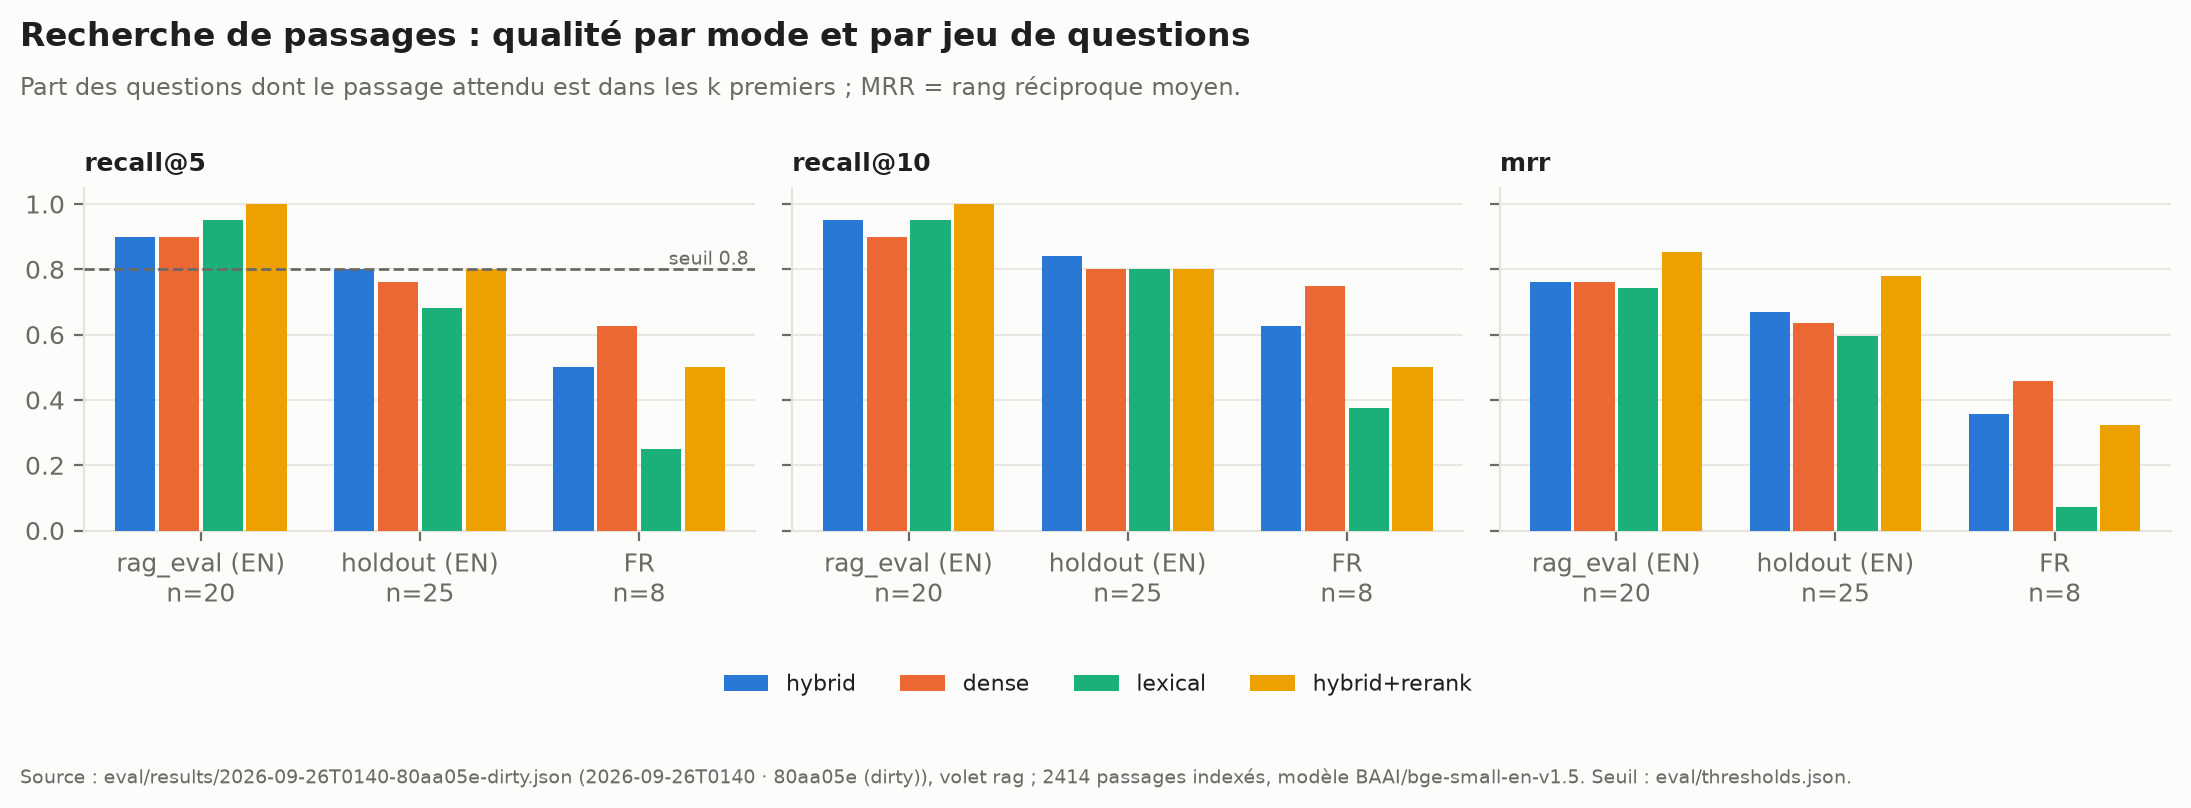
\includegraphics[width=\linewidth]{eval_retrieval.png}
\caption{The numbers of table~\ref{tab:eval}, plotted by \cmd{pdb plot eval} from the bench's
JSON report. The dashed line is the acceptance threshold (recall@5 $\geq$ 0.8).}
\label{fig:evalretrieval}
\end{figure}

\paragraph{Reading the results.}
\begin{itemize}
  \item \emph{The holdout falls below the threshold.} With 101 papers, no mode reaches a
    recall@5 of 0.8 on the holdout any more: the best, hybrid with reranking, drops from 0.80
    to 0.72, i.e.\ two questions fewer. The dev set also loses (1.00 $\rightarrow$ 0.90), as
    does French (0.50 $\rightarrow$ 0.38). This is the most important result of this run,
    and its cause is not established: the corpus more than doubled, which adds passages close
    to the expected ones; tables are now indexed by rows; and the search code was
    restructured. The only change measured in isolation, table chunking, changes neither the
    dev nor the holdout. The planned diagnosis replays the sets on the index restricted to
    the 45 papers of the reference run, then the old code on the current corpus, to separate
    the effect of the corpus from that of the code. The threshold is not lowered, and nothing
    is tuned on the holdout.
  \item \emph{The dev set was optimistic.} On the holdout, recall@5 loses 12 to 29 points
    depending on the mode, and lexical is the weakest. This confirms the expected bias: on
    the dev set, the expected sections had been chosen by keywords, which favoured \gl{BM25}{BM25}.
  \item \emph{Reranking remains the best mode in English}, on both sets. It no longer
    compensates, on its own, for the competition of the new papers.
  \item \emph{Real holdout failures} (with reranking): radiation tolerance (two questions),
    quantisation-aware training, memory of past examples, dataset distillation, and the two
    table questions (autoencoder resources in an hls4ml paper, FINN prototypes). For these two,
    the initial finding (``the text of a table is reduced to its caption'') no longer holds:
    since Docling, these tables have a body and are short enough not to be split. The failure
    comes from vocabulary: the question says ``resource utilization'', ``throughput'',
    ``autoencoder''; the table says ``LUT'', ``Thr.put'', ``AE''. Prefixing table passages with
    the paper title was tried, and does not help.
  \item \emph{In French, lexical collapses} (recall@5 of 0.00), and the \gl{index}{dense index} holds up
    better, although the model is not designed as multilingual. Reranking, trained on
    English \gl{MSMARCO}{MS MARCO}, degrades the ranking. The \gl{GPU}{GPU} engine (section~\ref{sec:qwen}) did much
    better on this set.
  \item \emph{Decisions.} Hybrid remains the default mode of \cmd{pdb search}, because
    reranking degrades French, following a rule set before the measurement. \cmd{/paper-ask}
    enables it, because it always phrases its queries in English and the rank of the first
    correct answer matters when only 2 or 3 passages are opened.
\end{itemize}

In an earlier measurement (25/09/2026, dev set), the \cmd{all-MiniLM-L6-v2} model reached a
recall@5 of 0.75 in dense mode versus 0.90 for bge-small, which motivated choosing the
latter. The acceptance threshold is a recall@5 of at least 0.8 in English.

\subsection{Detecting that a question falls outside the corpus}
\label{sec:horscorpus}

Can one tell, without an LLM, that the base does not cover a question? Two sets of 10
out-of-corpus questions (protein folding, blockchain, etc.) were written: one for
calibration, the other for validation. The second was written before any cross-encoder
measurement. Two signals are measured: the best cosine of dense retrieval, and the best
cross-encoder score over the top 3 passages. For each, the threshold is chosen on the
calibration data (dev set and first out-of-corpus set, from which a question half-covered by
the corpus was removed) by maximising balanced accuracy, then applied as is to the
validation data (holdout and second out-of-corpus set). The adoption rule was set before the
measurement: on validation, at least 80~\% of out-of-corpus questions flagged, and at most
5~\% of corpus questions.

\begin{table}[ht]
\centering
\caption{``Out-of-corpus'' signal: share of questions flagged on validation (10
out-of-corpus questions, 25 holdout questions), fpga base, 101 papers.}
\label{tab:horscorpus}
\small\setlength{\tabcolsep}{4pt}
\begin{tabular}{@{}p{5.6cm}cccc@{}}
\toprule
Signal & Threshold & Out-of-corpus flagged & Corpus wrongly flagged & Adopted \\
\midrule
cosine, initial hand-set threshold & 0.60 & 0.00 & 0.00 & -- \\
cosine, calibrated threshold & 0.78 & 0.80 & 0.20 & no \\
cross-encoder, calibrated threshold & 2.12 & 0.90 & 0.32 & no \\
\midrule
Qwen3-Reranker-4B, 28 papers (section~\ref{sec:qwen}) & 0.96 & 1.00 & 0.16 & no \\
\bottomrule
\end{tabular}
\end{table}

No signal meets the rule. With bge-small, an off-topic question gets a cosine as high as a
relevant one: the initial calibration, made on a few queries, did not hold, and the warning
never fired. The cross-encoder separates the medians better, but some corpus questions score
very low, often those where retrieval already fails. The warning was therefore removed from
\cmd{pdb search}. The GPU engine's reranker is the signal closest to the
rule: it flags all 10 out-of-corpus questions, but also 4 of the 25 holdout questions
(16~\%, for 5~\% allowed). It is not adopted either. The answer came from elsewhere: when it
is the agent that judges, from the content of the passages read, it recognises the
out-of-corpus questions (section~\ref{sec:answers}).

\subsection{Quotation checking}
\label{sec:evalverify}

The bench draws 40 random passages (fixed seed) and builds four kinds of quotations: an
exact sentence, which must be accepted; the same sentence with one word replaced, then with
one number changed, and a sentence from another paper, which must be rejected. ``Accepted''
means a zero exit code (\cmd{OK} or \cmd{APPROX} in the cited passage).

\begin{table}[ht]
\centering
\caption{Acceptance rate of \cmd{pdb verify}, before and after the number check. ``Before'':
28-paper run; ``After'': 03/10 run on 101 papers, whose random draw differs (33 sentences
with a changeable number instead of 38).}
\label{tab:verify}
\small
\begin{tabular}{@{}lccl@{}}
\toprule
Quotation & Before & After & Statuses after \\
\midrule
exact (40)             & 1.00 & 1.00 & 40 \cmd{OK} \\
number changed (33)    & \textbf{1.00} & \textbf{0.00} & 33 \cmd{NOMBRES} \\
word replaced (40)     & 0.97 & 0.97 & 39 \cmd{APPROX}, 1 \cmd{NOMBRES} \\
from another paper (40) & 0.00 & 0.00 & 40 \cmd{ABSENT} \\
\bottomrule
\end{tabular}
\end{table}

Before the check, \cmd{verify} accepted every quotation with a changed number, whereas the
agent's working rules rely on it to guarantee quoted numbers. A first version of the check
still let 6 through (a ``4'' recognised in ``6.4'', a ``2'' found elsewhere in the passage).
Requiring neighbouring words fixes both cases, but not all of them. On the drone base
(section~\ref{sec:drone}), the 03/10 run accepts, for the first time, a quotation with a
changed number: ``before step~2'' instead of ``before step~4'', in a passage that contains
``in step~2 and~3'' elsewhere. The changed number and its neighbouring word do exist in the
passage, but not at that place. This case is not fixed; it shows that the check guarantees
the presence of each number with its immediate context, not its position in the sentence.
Also still unhandled: a \emph{word} replaced far from any number still yields \cmd{APPROX}.
That is why \cmd{/paper-ask} keeps an \cmd{APPROX} quotation only when presented as a
paraphrase.

\subsection{Timings}

\begin{table}[ht]
\centering
\caption{Timings measured on the fpga base (8\,601 passages; medians of 3 repetitions, CPU
without GPU).}
\label{tab:temps}
\small
\begin{tabularx}{\linewidth}{@{}Ll@{}}
\toprule
Measurement & Value \\
\midrule
Extraction outside GROBID, per paper (TEI $\rightarrow$ text, ligatures, tables) & 0.01 to 0.13\,s \\
Index loading (8\,601 passages, 17\,MB) & 0.52\,s \\
bge-small encoding & 18 passages/s; full index $\approx$ 491\,s \\
Warm \cmd{search}, p50 / p95: lexical & 25 / 31\,ms \\
\quad dense & 117 / 146\,ms \\
\quad hybrid & 115 / 168\,ms \\
\quad hybrid + reranking & 1\,430 / 1\,782\,ms \\
Warm \cmd{verify} & 2\,ms \\
Cold commands, Python start-up included: \cmd{status} & 0.61\,s \\
\quad \cmd{bench}, \cmd{paper} & 0.09 and 0.08\,s \\
\quad \cmd{show} & 0.75\,s \\
\quad \cmd{search} & 6.6\,s \\
\bottomrule
\end{tabularx}
\end{table}

The cost of a search comes almost entirely from start-up (PyTorch import, model loading):
6.6\,s cold versus 0.1\,s warm. This is the real cost of a call by the agent, which launches
a command each time. With 2.5 times more passages than in the 28/09 run, warm search timings
have barely moved, and index loading goes from 0.29 to 0.52\,s. The \cmd{verify} time, which
had gone from 4 to 246\,ms without explanation, is back to 2\,ms.

\subsection{Real end-to-end trial}

Question asked to \cmd{/paper-ask}, on the 28-paper corpus: ``how do the papers measure
power, and is it comparable?''. The agent chained one \cmd{bench} query (57 rows, 8 papers),
one search of 10 passages, reading 3 of them, 7 quotation checks and 8 identity queries. The
whole amounts to about 9\,kB read, i.e.\ about 2\,500 tokens, without opening any full text.
All 7 verbatim quotations came back \cmd{OK} at the first attempt. Retrieval found in one
query the four measurement protocols of the corpus (PMBus and wall socket, multimeter at the
board input, \cmd{tegrastats}, idle power measured before the tests). The Read / Inferred /
Not found structure brought out two points to check in the base itself, including a paper
that describes a careful measurement while no power row had been entered. The trial also
revealed two defects, fixed since and each covered by a test: a short identifier truncated
for a compound author name, and an aggregation that required an external script (hence
\cmd{bench --count}). This trial was a single one, judged by the agent that ran it; the next
section replaces it with a repeatable evaluation.

\subsection{Evaluating the written answer}
\label{sec:answers}

The previous parts measure the ranking of passages. They do not say whether the final answer
recognises an out-of-corpus question, whether its quotations hold, or whether it finds the
expected sources and values. \cmd{pdb eval --answers} measures this, still without an LLM:
the answers are produced separately, then scored.

\paragraph{Protocol.} Each question of an answer set carries a category, the
\gl{exigence}{requirements} of a complete answer, the expected sources (sections or papers), the expected
values with their unit, and the expected verdict. There are four categories: a sourced fact
in a paper (\emph{simple}), values with their conditions (\emph{numerical}), a synthesis
across several papers (\emph{synthesis}), and a question close to the theme that the corpus
does not cover (\emph{absent}: polyps in endoscopy, sign language, sonar, EEG\ldots, checked
absent by full-text search). The \cmd{/eval-answers} skill hands each question to a subagent
that receives only its text, no category, no sources, no expected verdict, and that answers
with \cmd{/paper-ask --record}. The recorded answer is a list of statements marked read or
inferred, each with its citations and their excerpts. The bench computes the accuracy of the
verdict, the share of accepted citations (\cmd{verify} returns \cmd{OK} or \cmd{APPROX} in
the cited passage, or the cited section is among the sources of the paper's \cmd{bench}
rows), the share of ``read'' statements without any accepted citation, and the recall of the
expected sources and values. A grid of human ratings (requirements, support, conditions,
limitations, from 0 to 2) is planned: the automatic checks verify that the excerpts exist,
not that they support the sentence.

\paragraph{First runs.} The starting sets of the fpga base have 12 development and 12
held-out questions, 3 per category, written by the author of the code. Two runs were made on
02/10/2026, one answer per question, by Sonnet subagents; the second with the version of
\cmd{/paper-ask} that states the requirements and the sufficiency verdict
(section~\ref{sec:paperask}). Both runs were made in a degraded configuration: the dense
retrieval and reranking models could not be downloaded from the container, so retrieval was
lexical only (table~\ref{tab:answers}).

\begin{table}[ht]
\centering
\caption{Written answers, fpga base (12 + 12 questions, lexical retrieval only). In
parentheses: first run, before the sufficiency verdict.}
\label{tab:answers}
\small
\begin{tabularx}{\linewidth}{@{}l*{5}{>{\centering\arraybackslash}X}@{}}
\toprule
Set & Correct verdict & Accepted citations & Unsupported statements & Expected sources & Expected values \\
\midrule
dev (12)     & 0.75 (0.83) & 1.00 (0.96) & 0.00 (0.02) & 0.87 (0.91) & 1.00 (1.00) \\
holdout (12) & 0.83 (0.92) & 1.00 (1.00) & 0.00 (0.00) & 0.50 (0.67) & 1.00 (1.00) \\
\bottomrule
\end{tabularx}
\end{table}

\begin{itemize}
  \item \emph{Out of corpus.} In both runs, the 6 \emph{absent} questions are recognised as
    such, and no corpus question is wrongly declared absent. The answers say that the base
    does not cover the topic, without filling the gap with general knowledge. This is what
    no retrieval score could achieve (section~\ref{sec:horscorpus}). With 6 questions, it is
    a signal, not a measurement.
  \item \emph{Citations.} In the second run, all citations are accepted and every ``read''
    statement carries at least one.
  \item \emph{Synthesis.} This is the weak category: 3 correct verdicts out of 6 in the first
    run, 2 in the second. The agent answers \cmd{partiel} where the set expects \cmd{suffisant},
    because a requirement of the question (memory budget of each method, comparability of the
    measurements) is only partly covered by the corpus. These answers are defensible; the
    boundary between sufficient and partial is to be clarified in the set rather than in the
    skill. The drop in correct verdicts in the second run comes from there, and from one
    answer where the new rule (a \cmd{suffisant} verdict requires all requirements to be
    covered) corrects an inconsistency of the first run.
  \item \emph{Variance.} 22 verdicts out of 24 are identical from one run to the other: the
    bench is stable enough to compare versions of the skill on verdicts. It is not yet stable
    on the recall of sources (0.67 $\rightarrow$ 0.50 on the holdout with no change to
    retrieval). This recall also underestimates the answers: most gaps come from an
    equivalent source (the \cmd{bench} row or the table passage rather than the expected text
    section).
\end{itemize}
No threshold is set yet: what is missing is a run with hybrid retrieval and reranking,
larger sets (40 development and 60 held-out questions per base, written or reviewed by a
third party) and the human ratings.

\subsection{A second corpus: the drone base}
\label{sec:drone}

The drone base (section~\ref{sec:bases}) has its own question sets, written with the same
protocol on its first 73 papers: 20 development questions, 20 held-out, 8 in French and two
sets of 10 out-of-corpus questions. Thresholds are those of the fpga base, fixed before the
first run. Table~\ref{tab:drone} compares the two bases (runs of 03/10/2026 at commit 3925690).

\begin{table}[ht]
\centering
\caption{Evaluation bench on the two bases that have question sets, on 03/10/2026
(recall@5 unless stated).}
\label{tab:drone}
\small
\begin{tabularx}{\linewidth}{@{}Lll@{}}
\toprule
Measure & fpga (101 papers) & drone (87 papers) \\
\midrule
Passages & 8\,601 & 5\,361 \\
Text coverage: mean / minimum & 0.90 / 0.57 & 0.91 / 0.77 \\
Tables with a body & 0.78 & 0.79 (0.90 on the 73 GROBID papers) \\
Header: title / year / DOI & 0.87 / 0.47 / 0.65 & 0.92 / 0.64 / 0.70 \\
\cmd{benchmarks.csv} values found in the cited table & 0.70 (1\,044) & 0.62 (739) \\
Dev, hybrid / hybrid + reranking & 0.80 / 0.90 & 0.90 / 1.00 \\
Held-out, hybrid / hybrid + reranking & 0.68 / 0.72 (25 q.) & 0.90 / 0.95 (20 q.) \\
Held-out, MRR hybrid + reranking & 0.62 & 0.89 \\
French, hybrid + reranking & 0.38 & 0.50 \\
Low relevance (\cmd{cos}): out-of-corpus / in-corpus flagged & 0.80 / 0.20 & 1.00 / 0.10 \\
\cmd{verify}: exact / word replaced / number altered / other paper & 1.00 / 0.97 / 0.00 / 0.00 & 1.00 / 0.82 / 0.03 / 0.00 \\
\bottomrule
\end{tabularx}
\end{table}

The reading calls for caution:
\begin{itemize}
  \item \textbf{The drone held-out set meets its threshold}, but one cannot conclude that
    retrieval works better there. The drone corpus is more heterogeneous (detection, tracking,
    neuromorphic, drone racing): a distinctive fact has fewer close neighbours than in a
    corpus centred on accelerators. Two expectations were also widened after reading the
    returned passages. On 20 questions, 0.05 is one question. Between 28/09 and 03/10, with
    14 more papers and 836 more passages, hybrid loses one question on each English set, and
    reranking loses none.
  \item \textbf{Failures are of the same kind} as on the fpga base: a table (idle power of
    several boards) missed by every mode, and half of the French questions.
  \item \textbf{Low relevance remains unusable}: the cosine flags every out-of-corpus
    validation question, but also 2 of the 20 held-out questions, above the 5~\% of false
    alarms tolerated.
  \item \textbf{Tables.} Running Docling on this base (29/09) raised the share of tables with a
    body from 0.71 to 0.90 and the values found in their table by 3 points, with a constant
    corpus: this is the first measured gain of Docling on these values. The share falls back
    to 0.79 on 87 papers because the 14 papers added since were added without their PDF:
    extracted by PyMuPDF without GROBID, they have no table with a body (0 out of 50) and
    cannot go through Docling.
  \item \textbf{\cmd{verify}} accepts one quotation with a changed number out of 30, and the
    corresponding threshold is no longer met (section~\ref{sec:evalverify}).
\end{itemize}

\paragraph{The stage base.} It has no question sets yet: the bench only measures its
extraction (56 papers, 3\,640 passages, run
\cmd{bases/stage/eval/results/2026-10-03T2344-3925690.json}). Mean coverage is 0.91 (minimum
0.61 for the scanned reprint of Mahalanobis, 1936), but only 71~\% of the 254 tables have a
body, none having gone through Docling, and only 42~\% of the 112 values of
\cmd{benchmarks.csv} are found in the cited table (57~\% anywhere in the text): these rows are
the first to reread. It is also the only base where unrepaired ligatures remain (0.37 per
10\,000 words). Without question sets of its own, the bench until now silently fell back on
the fpga base's questions, whose recall makes no sense here: this fallback must become a
warning.

\subsection{Synthetic benchmark (\cmd{pdb synth})}
\label{sec:synth}

The previous sets are small and written by the author of the system. \cmd{bin/pdb synth}
prepares a larger evaluation, kept apart from the working base (\cmd{.cache/bench/}):
\begin{itemize}
  \item a \emph{frozen corpus} of 200 papers, with neighbouring topics as distractors;
    question anchor passages are screened for \gl{FPGA}{FPGA}, embedded \gl{AI}{AI} and hardware acceleration,
    excluding introductions and background;
  \item \emph{local generation} of questions by an open model (Qwen3.8-27B quantised to Q6,
    served by llama.cpp on the same RTX 5090), as schema-constrained JSON with a fixed seed;
    the identity of the served model and every quotation are checked;
  \item \emph{validation without human labels}: two independent sessions of an LLM (Codex
    for the 200 reference questions, then Claude Code in non-interactive mode,
    \cmd{claude -p}) check each question;
  \item \emph{quotas}: 40 single-passage, 40 numerical, 50 cross-paper, 30 within-paper, 20
    table and 20 missing-evidence questions; a 40~\% development, 60~\% test split over
    disjoint paper sets, balanced between English and French, and 40 questions declined into
    translated and terse variants;
  \item \emph{ablations}: the four retrieval modes of the GPU engine and the two CPU modes of
    \cmd{pdb search} on the same questions, then agent variants run in a sandbox (bubblewrap,
    read-only tools, read-only corpus), scored by an LLM judge.
\end{itemize}
Automatically produced notes and numerical transcriptions form a separate \emph{enriched}
corpus, never used to write reference answers; a \gl{benchmark}{benchmark row} is kept there only if each
of its numbers appears in the cited section. The protocol and its tests are in place; its
results are not available yet and are therefore not reported here.

\subsection{Threats to validity}

\begin{itemize}
  \item The sets are small: on 25 questions, a difference of 0.04 is a single question, and
    no difference below two questions is readable. The holdout tuned no parameter, but it was
    written, like the dev set, by the author of the system. Questions written by a third
    party are needed to confirm the differences. The second corpus
    (section~\ref{sec:drone}) shows that the trends are not tied to a single corpus, but its
    questions were written by the same author.
  \item The sets did not follow the growth of the bases: written for 45 and 73 papers, they
    now query less than half of the fpga corpus, and the stage base has none.
  \item Expected sections are chosen by text pattern. This is an approximation: a correct
    answer phrased differently, or found in a paper added after the set was written, counts
    as a failure.
  \item The ground truth for tables only covers values taken into \cmd{benchmarks.csv}, and the
    rate of tables ``with a body'' says nothing about the accuracy of the cells.
  \item The written answers are scored automatically on 24 questions, with lexical retrieval
    only, and the human ratings have not been assigned yet: the validity of the citations is
    checked, not whether they support the sentence.
  \item The comparison of the two engines is on the 28-paper corpus and on the original
    \cmd{pdb rag} chain; it was not redone with the engine built into \cmd{pdb search}, nor on
    the current corpus.
  \item The savings from delegation rest on an estimate, calibrated by a single paired trial,
    on a single task, with no scoring of quality.
  \item The synthetic benchmark will have its own biases: questions generated by an LLM,
    validated and scored by other LLMs. It will measure this frozen corpus and this task
    distribution, not research work in general.
\end{itemize}

\section{Limitations and outlook}

\begin{itemize}
  \item \textbf{Scaling.} From 45 to 101 papers, the \gl{holdout}{holdout} \gl{recall}{recall@5} with \gl{reranking}{reranking}
    goes from 0.80 to 0.72, below the threshold. Before any tuning, the effect of the corpus
    must be separated from that of the code, by replaying the sets on the common sub-corpus
    and the old code on the current corpus. The next plan is specified: question sets of each
    base's own, with no silent fallback; a size proportional to the corpus (a holdout of at
    least 40 questions or half the number of papers); quotas per axis of the base and per
    question type (tables, several papers); questions proposed by the synthetic-benchmark
    chain and reviewed by a human; a new reference run each time the corpus grows by 25~\%;
    and bootstrap confidence intervals, so that a difference is flagged only if it falls
    outside them.
  \item \textbf{Tables.} They remain the most fragile part of extraction: 22~\% of the tables
    of the fpga base have no body, about 40~\% of those that have one are flagged by a quality
    signal, and \gl{OCR}{OCR}'d tables are of uneven quality. Tables are hard to retrieve, now for a
    vocabulary reason (header abbreviations) more than for chunking; a per-base glossary of
    abbreviations or multiple queries are the leads. Still to do: a skill to reread flagged
    tables, starting with those cited by \cmd{benchmarks.csv}, a ground truth of about twenty
    hand-annotated tables, and OCR targeted at the table area rather than the whole PDF. A
    re-extraction (\cmd{ingest --reparse}) also undoes some ligature repairs: to be fixed
    before any mass re-extraction.
  \item \textbf{Comparisons.} \cmd{bench --comparable} says which rows compare along one axis.
    A \cmd{pdb compare} command, specified, will compare along two axes (throughput versus
    power, at equal metric and dataset), give a confidence level per group and explain each
    excluded row. The optional columns remain to be filled: no row carries its passage yet.
  \item \textbf{Atomic evidence.} Only one paper has its \cmd{claims.jsonl}. The others remain
    to be produced, to be indexed as pointers to their passage, and to be read by
    \cmd{/paper-ask}, which should gain on synthesis questions.
  \item \textbf{Answers.} Missing are a run of the answers with hybrid retrieval and reranking,
    larger sets reviewed by a third party, sets for the drone and stage bases, and the human
    ratings.
  \item \textbf{Out-of-corpus questions.} No retrieval score reliably says that the base does
    not cover the topic; the agent's sufficiency verdict manages it on the 6 questions
    tested, which remains to be confirmed on a larger set.
  \item \textbf{Verification.} \cmd{verify} rejects changed numbers when the number and its
    neighbours are not found elsewhere in the passage, but not in the opposite case
    (section~\ref{sec:evalverify}), and a word replaced far from any number still passes as a
    paraphrase (\cmd{APPROX}). The check of \cmd{rag check-answer}, on the GPU route, does not
    check numbers yet.
  \item \textbf{Metadata.} A publisher template \gl{DOI}{DOI} (MDPI) is not yet rejected at extraction;
    it is fixed by hand in the base, but a new paper from the same publisher would inherit
    it.
  \item \textbf{Language.} The corpus and the default model are in English, and \gl{CPU}{CPU}
    retrieval loses a lot in French (recall@5 of 0.38 with reranking). The \gl{GPU}{GPU} engine
    retrieved all 8 French questions, at the price of a GPU. Specified leads: systematically
    translate the query and merge the results, evaluate a multilingual model alongside the
    current one, and raise the French set to 30 questions per base.
  \item \textbf{Provenance.} Nothing keeps track of the state of the corpus on which an answer
    was written: after a reindex, one cannot know what it was based on. A corpus fingerprint
    and an answer log are planned.
  \item \textbf{Latency.} About 7\,s per cold \cmd{search}, versus 0.1\,s warm, mostly due
    to the PyTorch import and model loading; \cmd{show} and \cmd{verify}, which do without
    them, answer in under a second. A resident process, for example an \gl{MCP}{MCP} server exposing
    the same commands, would pay this cost only once and would let other applications use
    the base. The same argument applies to the GPU engine, which reloads its models for
    each query (3 to 4\,s).
  \item \textbf{Genericity.} The same code serves three bases (section~\ref{sec:bases}), one of
    them with no hardware measurement at all, and a new one is created with \cmd{pdb base new}.
    The mandatory columns of \cmd{benchmarks.csv} (\gl{FPS}{FPS}, \gl{GOPS}{GOPS}, \gl{FPGA}{FPGA} resources) remain
    marked by the original domain: out of 100 rows, the stage base has no FPGA resource and
    two throughputs; it reports its results as accuracy or prediction error. The optional
    columns and the per-base \cmd{plot} block made the schema more flexible without making it
    configurable.
\end{itemize}

\section{Conclusion}

PaperDatabase shows that a modest research corpus can be made usable by an \gl{LLM}{LLM} \gl{agent}{agent} without
a database or an external service: well-structured text files, a table of sourced numbers
and a deterministic hybrid search are enough. Generation stays with the agent, but
everything it quotes can be replayed and checked by a command. The cost of a sourced answer
drops by an order of magnitude compared with reading full texts, and delegating reading to
less expensive subagents reduces the bill further, by 41~\% in the single paired trial.

The evaluation bench showed the value of measuring what one believes settled: an optimistic
question set, a warning that never fired, a check that let wrong numbers through, and then,
on remeasuring, a retrieval that loses recall when the corpus doubles. This last point is the
main open problem. The evaluation of the written answers brought the opposite result: where no
score could tell that a question falls outside the corpus, the agent says so when it is made
to confront each requirement of the question with the passages read. The same code serves
three isolated bases, on which the bench finds the same strengths and the same weaknesses.
Next steps are the diagnosis of the recall drop and question sets at the scale of the bases,
questions written by a third party, human ratings of the answers, better retrieval within
tables, comparison along two axes and a resident engine that avoids reloading models for each
query.

\bibliographystyle{plainnat}
\bibliography{refs}

\appendix
\section{Glossary of acronyms}
\label{sec:acronymes}

\begin{center}
\small
\begin{tabularx}{\linewidth}{@{}lL@{}}
\toprule
Acronym & Meaning \\
\midrule
\hypertarget{gl:AI}{AI} & artificial intelligence \\
\hypertarget{gl:API}{API} & Application Programming Interface \\
\hypertarget{gl:BF16}{BF16} & bfloat16, 16-bit floating-point format \\
\hypertarget{gl:BM25}{BM25} & Best Matching 25, scoring function of lexical retrieval \\
\hypertarget{gl:BRAM}{BRAM} & Block RAM, on-chip memory of an FPGA \\
\hypertarget{gl:CPU}{CPU} & Central Processing Unit \\
\hypertarget{gl:CSV}{CSV / TSV} & Comma- / Tab-Separated Values \\
\hypertarget{gl:DOI}{DOI} & Digital Object Identifier, persistent identifier of a publication \\
\hypertarget{gl:DSP}{DSP} & Digital Signal Processing: arithmetic block (multiply-accumulate) of an FPGA \\
\hypertarget{gl:FPGA}{FPGA} & Field-Programmable Gate Array \\
\hypertarget{gl:FPS}{FPS} & Frames Per Second \\
\hypertarget{gl:FTS5}{FTS5} & Full-Text Search version 5, SQLite full-text index \\
\hypertarget{gl:GOPS}{GOPS} & Giga Operations Per Second \\
\hypertarget{gl:GPU}{GPU} & Graphics Processing Unit \\
\hypertarget{gl:GROBID}{GROBID} & GeneRation Of BIbliographic Data, structure extractor for PDF papers \\
\hypertarget{gl:INT8}{INT8} & 8-bit integers (quantisation) \\
\hypertarget{gl:JSON}{JSON} & JavaScript Object Notation \\
\hypertarget{gl:LLM}{LLM} & Large Language Model \\
\hypertarget{gl:LUT}{LUT} & Look-Up Table, elementary logic cell of an FPGA \\
\hypertarget{gl:MCU}{MCU} & Microcontroller Unit \\
\hypertarget{gl:MCP}{MCP} & Model Context Protocol, protocol exposing tools to an LLM agent \\
\hypertarget{gl:MRR}{MRR} & Mean Reciprocal Rank of the first correct answer \\
\hypertarget{gl:MSMARCO}{MS MARCO} & Microsoft MAchine Reading COmprehension, passage-retrieval dataset \\
\hypertarget{gl:nDCG}{nDCG} & normalized Discounted Cumulative Gain, ranking quality \\
\hypertarget{gl:NMS}{NMS} & Non-Maximum Suppression, removal of duplicate detection boxes \\
\hypertarget{gl:OCR}{OCR} & Optical Character Recognition \\
\hypertarget{gl:PDF}{PDF} & Portable Document Format \\
\hypertarget{gl:RAG}{RAG} & Retrieval-Augmented Generation \\
\hypertarget{gl:RRF}{RRF} & Reciprocal Rank Fusion \\
\hypertarget{gl:SHA}{SHA-1} & Secure Hash Algorithm 1, hash of a text \\
\hypertarget{gl:TEI}{TEI} & Text Encoding Initiative, XML output format of GROBID \\
\hypertarget{gl:YOLO}{YOLO} & You Only Look Once, family of object detectors \\
\bottomrule
\end{tabularx}
\end{center}

\section{Glossary}
\label{sec:lexique}

\begin{center}
\small
\begin{tabularx}{\linewidth}{@{}lL@{}}
\toprule
Term & Meaning in this document \\
\midrule
\hypertarget{gl:agent}{agent} & LLM that calls tools (file reading, commands) to carry out a task; here Claude Code \\
\hypertarget{gl:benchmark}{benchmark row} & one configuration reported by a paper (model, platform, precision, throughput, power\ldots), with its source section, in \cmd{benchmarks.csv} \\
\hypertarget{gl:passage}{chunk, passage} & section fragment indexed for retrieval, identified by \cmd{<paper>\#<section>.<k>} \\
\hypertarget{gl:crossenc}{cross-encoder} & model that scores a query and a passage together; used for reranking \\
\hypertarget{gl:exigence}{requirement} & what a complete answer must establish (value, platform, condition\ldots); status \cmd{couvert}, \cmd{partiel} or \cmd{absent} \\
\hypertarget{gl:embedding}{embedding} & vector representing the meaning of a text; close texts have close vectors \\
\hypertarget{gl:fiche}{reading note (\cmd{fiche})} & critical reading of a paper (\cmd{fiche.md}): problem, method, results, limitations, relevance \\
\hypertarget{gl:hook}{hook} & command that Claude Code launches by itself at a given moment (here, at the end of each subagent) \\
\hypertarget{gl:holdout}{holdout} & reserved question set, never used to tune any parameter \\
\hypertarget{gl:index}{dense / lexical index} & index by embeddings (meaning) / by exact words (BM25, FTS5) \\
\hypertarget{gl:gap}{gap} & area the corpus does not cover, recorded in \cmd{gaps.md} \\
\hypertarget{gl:nr}{\texttt{n/r}} & ``not reported'': value absent from the paper, never estimated \\
\hypertarget{gl:scope}{power scope} & what a power measurement covers (chip, board, estimate), \cmd{power\_scope} column \\
\hypertarget{gl:claim}{atomic evidence (claim)} & one statement of a paper, with its source passage and the exact excerpt that carries it, in \cmd{claims.jsonl} \\
\hypertarget{gl:preprint}{preprint} & paper released without peer review (arXiv) \\
\hypertarget{gl:recall}{recall@$k$} & share of questions for which an expected section is among the top $k$ passages \\
\hypertarget{gl:paperk}{paper@$k$} & share of questions for which an expected paper is among the top $k$ passages \\
\hypertarget{gl:reranking}{reranking} & reordering of the top results by a more expensive model \\
\hypertarget{gl:skill}{skill} & written procedure the agent follows for a task (\cmd{/paper-ask}, \cmd{/paper-fiche}\ldots) \\
\hypertarget{gl:sousagent}{subagent} & agent launched by the main agent for a delimited task, without its context, often on a less expensive model \\
\hypertarget{gl:toolflow}{toolflow} & tool chain turning a neural network into a hardware accelerator (FINN, hls4ml\ldots) \\
\hypertarget{gl:verdict}{sufficiency verdict} & at the head of an answer: \cmd{suffisant} (all requirements covered), \cmd{partiel} or \cmd{absent} (none) \\
\bottomrule
\end{tabularx}
\end{center}

\section{Commands}

\begin{center}
\small
\begin{tabularx}{\linewidth}{@{}lL@{}}
\toprule
Command & Effect \\
\midrule
\cmd{bin/pdb status [--tables]} & state of the base and next actions; table quality signals \\
\cmd{bin/pdb add <arxiv | doi | pdf>} & acquisition, ingestion and reindexing \\
\cmd{bin/pdb ingest [--force | --reparse]} & (re)extraction of the PDFs in \cmd{inbox/} \\
\cmd{bin/pdb ingest --reparse --tables docling [--ocr]} & bodiless tables handed to Docling \\
\cmd{bin/pdb reindex} & \cmd{INDEX.md}, \cmd{external\_refs.csv}, passage index \\
\cmd{bin/pdb bench [filters]} & filters \cmd{benchmarks.csv}, source columns always shown \\
\cmd{bin/pdb bench --check | --comparable | --add-columns} & values found in their passage; comparable groups; optional columns \\
\cmd{bin/pdb claims <id> [--check]} & atomic evidence of a paper and its check \\
\cmd{bin/pdb paper <id | word>…} & identity of one or more papers \\
\cmd{bin/pdb search "<q>"} & ranked passages (hybrid, optional \cmd{--rerank}; \cmd{--gpu} / \cmd{--cpu}) \\
\cmd{bin/pdb gpu [on | off]} & state of the GPU engine; enabling it for the machine, back to the CPU \\
\cmd{bin/pdb show <chunk\_id>} & exact text of a passage \\
\cmd{bin/pdb verify <chunk\_id> "<quote>"} & checks a quotation \\
\cmd{bin/pdb cites | cited-by <id>} & internal citation graph \\
\cmd{bin/pdb discover} & candidates to add, via OpenAlex \\
\cmd{bin/pdb plot [bench | eval | corpus | all]} & static figures and \cmd{figures/manifest.json} \\
\cmd{bin/pdb plot --check | --stale} & \cmd{plot} block proposed for the base; stale figures only \\
\cmd{bin/pdb viz} & local corpus visualisation \\
\cmd{bin/pdb rag index | search | evidence | benchmarks} & GPU engine (Qwen3): index, search, evidence, numbers \\
\cmd{bin/pdb rag acquire | approve | check-answer} & open-access acquisition, import after approval, answer check \\
\cmd{bin/pdb synth <step>} & synthetic benchmark (corpus, generation, validation, ablations, report) \\
\cmd{bin/pdb base list | new | register | use} & registered bases, creation, registration, default base \\
\cmd{bin/pdb base info | check} & profile and axes of a base; effect of the \cmd{base.json} rules \\
\cmd{bin/pdb base scan | import <base>:<id>} & useful papers from another base; copy of a paper \\
\cmd{bin/pdb --base <name> <command>} & act on a base other than that of the current folder \\
\cmd{bin/pdb test} & unit tests \\
\cmd{bin/pdb eval [--extract | --rag | --speed]} & evaluation bench, by part or complete \\
\cmd{bin/pdb eval --save | --compare} & saves a report; compares with the latest one and the thresholds \\
\cmd{bin/pdb eval --rag --gpu} & retrieval evaluated with the GPU engine, same keys \\
\cmd{bin/pdb eval --questions | --answers <run>…} & questions only; scoring of the written answers \\
\cmd{bin/pdb agents [--report | --scan | --mark]} & subagent log and cost, savings from delegation \\
\midrule
\cmd{/paper-add}, \cmd{/paper-fiche} & agent skills: addition; reading note and benchmark rows \\
\cmd{/paper-extract} & atomic evidence of a paper (\cmd{claims.jsonl}) \\
\cmd{/paper-ask}, \cmd{/paper-gaps}, \cmd{/paper-discover} & sourced answer with sufficiency verdict; gap map; discovery \\
\cmd{/eval-answers} & blindly produces the answers of a set, then has them scored \\
\cmd{/paper-research} & sourced answer with the GPU engine and open-access acquisition \\
\cmd{/base-profile} & proposed refinement of the base's profile and rules \\
\bottomrule
\end{tabularx}
\end{center}

\paragraph{Installation.} Python 3.12 and Docker (for GROBID):
\begin{lstlisting}
bash bin/setup.sh                                  # .venv and dependencies
.venv/bin/pip install -r requirements-embed.txt    # optional: dense retrieval
bin/pdb grobid start                               # GROBID on localhost:8070
bin/pdb add 2507.18174 && bin/pdb test
\end{lstlisting}

\end{document}
